%I need 12000 words~27 pages of introduction to my Licentiate as the literature review part, I think the space budget can go (roughly) like this:
%----------------------------------------------------------------------------------------
%    PACKAGES AND OTHER DOCUMENT CONFIGURATIONS
%----------------------------------------------------------------------------------------
\documentclass[paper=a4, fontsize=11pt]{scrartcl} % A4 paper and 11pt font size
\oddsidemargin=-0.54cm
\evensidemargin=-0.54cm
\topmargin=-1.2cm
\textwidth=17cm
\textheight=25cm
\usepackage[T1]{fontenc} % Use 8-bit encoding that has 256 glyphs
\usepackage{fourier} % Use the Adobe Utopia font for the document - comment this line to return to the LaTeX default
\usepackage[english]{babel} % English language/hyphenation
\usepackage{amsmath,amsfonts,amsthm} % Math packages
\usepackage{hyperref}
\makeatletter
\newcommand\urlfootnote@[1]{\footnote{\url@{#1}}}
\DeclareRobustCommand{\urlfootnote}{\hyper@normalise\urlfootnote@}
\makeatother
\usepackage{graphicx}
\usepackage{wrapfig}
\usepackage{caption}
\usepackage{sidecap}
\usepackage{subcaption}
\usepackage{float}
\usepackage{epstopdf}
\usepackage{titlesec}
\usepackage{verbatim}
\usepackage{amssymb}
\usepackage{amsmath}
\usepackage{natbib}

\makeatletter
\@addtoreset{section}{part}
\makeatother
\usepackage{fancyhdr} % Custom headers and footers
\pagestyle{fancyplain} % Makes all pages in the document conform to the custom headers and footers
\fancyhead{} % No page header - if you want one, create it in the same way as the footers below
\fancyfoot[L]{} % Empty left footer
\fancyfoot[C]{} % Empty center footer
\fancyfoot[R]{\thepage} % Page numbering for right footer
\renewcommand{\headrulewidth}{0pt} % Remove header underlines
\renewcommand{\footrulewidth}{0pt} % Remove footer underlines
\setlength{\headheight}{13.6pt} % Customize the height of the header

\numberwithin{equation}{section} % Number equations within sections (i.e. 1.1, 1.2, 2.1, 2.2 instead of 1, 2, 3, 4)
\numberwithin{figure}{section} % Number figures within sections (i.e. 1.1, 1.2, 2.1, 2.2 instead of 1, 2, 3, 4)
\numberwithin{table}{section} % Number tables within sections (i.e. 1.1, 1.2, 2.1, 2.2 instead of 1, 2, 3, 4)

\setlength{\parindent}{2em}
\setlength{\parskip}{1em}
%\setlength\parindent{0pt} % Removes all indentation from paragraphs - comment this line for an assignment with lots of text
%----------------------------------------------------------------------------------------
%    TITLE SECTION
%----------------------------------------------------------------------------------------

\newcommand{\horrule}[1]{\rule{\linewidth}{#1}} % Create horizontal rule command with 1 argument of height
\newcommand{\ignore}[1]{}

\title{    
\normalfont \normalsize 
%\textsc{Dark Cosmology Center\\Copenhagen - Denmark} \\ [25pt] % Your university, school and/or department name(s)
\horrule{0.5pt} \\[0.4cm] % Thin top horizontal rule
%\huge  Gravitational lensing and radio interferometers probe sub-galactic dark matter structure\\
%\huge  Probing dark matter substructure with gravitational lensing and radio interferometry\\
\huge Graviational lensing and radio interferometry as a probe of the small-scale structure of dark matter\\
%\large (story of my life) % The assignment title
\horrule{2pt} \\[0.5cm] % Thick bottom horizontal rule
}

\author{Saghar Asadi} % Your name

\date{\normalsize 2015 \\ Department of Astronomy \\ Stockholm University} % Today's date or a custom date

\pagestyle{empty}

\begin{document}

\maketitle % Print the title
\newpage
\tableofcontents
\newpage

\begin{abstract}
{\Large \bf Abstract}\\


Dark matter has been one of the great mysteries of physics since the early years of the 20$^\mathrm{th}$ century. Despite the numerous evidence for the dark matter constraining its poperties, the concordance model of cosmology -- accounting for dark matter as the second abundant component in the Universe -- is yet to describe the observed Universe at different scales simultaneously.

Gravitaional lensing is a well--known phenomenon due to the fact that gravity treats dark and luminous mass the same way. This gives gravitatioan lensing a unique advantage over many other observational methods to provide an independent test for the presence of dark structures of various size and mass. Strong lensing by a foreground object can produce multiple images of a background light source. Measurements of strong lens systems provide information about mass distribution of both the lens and the source. In order to study the structure inside dark matter halos of galaxies we need to look at a particular type of lens system where the foreground galaxy produces multiple images of the background light source, and the halo substructure presents itself as surface brightness perturbations in one of the lensed images.

Revealing small--scale surface brightness perturbations requires high--resolution imaging of lensed extended object, such as star--forming galaxies and radio jets. Radio interferometry is a tecchnique that connects an array of radio antennae to essentailly work as a single dish with the diameter as large as the maximum distance within the array. Therefore, arrays such as the European VLBI network and ALMA makes it possible to probe radio quasars and sub-mm galaxies with sub--milliarcsecond angular resolutions.

In this thesis, we simulate observations of multiply--lensed sources (radio quasars, and dusty star--forming galaxies) at $z \simeq 2$ with different (present and near--future) radio interferometers. These simulations are used to place constraints on various forms of suggested halo substructure within the lens halo. In {\bf paper I}, we derive the lowest mass that subhalos of various densities need to have in order to produce a detectable lensing effects on multiply--imaged quasars at three different frequencies. Using the mass resolution of different forms of subhalos, we propose the number of lens systems to investigate to place constraints on the contribution of each form of substructure in the mass of the parent halo. {\bf Paper II} focuses on similar simulations of sub--mm galaxies using ALMA, and the observational prospects of standard cold dark matter (CDM) subhalos. In this paper, we show that standard CDM subhalos in the sub--galactic mass range are detectable using high--frequency observations with ALMA. Besides, such observations would be able to tell the difference between the standard CDM subhalos and other dark compact objects, which in turn can place a constraint on the contribution of CDM subhalos in the mass of their host halo -- a quantity directly comparable to cosmological simulations.





 

\end{abstract}

\newpage
%----------------------------------------------------------------------------------------

\section{Dark matter}
Dark matter as the second dominant component of our Universe is thought to be made of non--baryonic, cold (i.e. non--relativistic), weakly interacting massive particles (WIMPs). Some of these characteristics are inferred from cosmological evidence. For instance, observation of small--scale cosmic structure indicates that the dark matter must be non--relativistic, while the measured abundance of light elements in the Universe along with the Big Bang Nucleosynthesis (BNN) results in the dark matter being non--baryonic. The ``missing matter'' in the Universe has presented itself both locally, i.e. in the galactic disk, and at the cosmic scale in the past century and even though the problem has been approached from the particle--physics point of view in addition to the cosmological one, it is still considered as one of the biggest challenges of both!

I start this chapter by briefing independent cosmological evidence for the presence of dark matter (in a decreasing physical scale order, which does not necessarily correspond to the historical order) and what each of them tell us about the nature and characteristics of dark matter. The chapter is finished by s review on the  current state of the dark matter followed by the detection methods currently used to approach the issue.
%In the end, I introduce the most competing alternative to the issue of the missing matter in the Universe, known as modifien Newtonian dynamics (MOND).

On the one hand, modern data suggests an insignificant amount of dark matter in the Solar vicinity which is made of baryonic but not luminous matter such as faint stars or Jupiter--like objects. In short, according to our current understanding of the Universe, dark matter is the dominant matter component of the Universe.

%----------------------------------------------------------------------------------------

\subsection{Why do we need dark matter?}
%(cosmological evidence)

%\subsubsection*{Independent measurement of the amount of baryons in the Universe}
The amount of baryons in the Universe could me measured with five independent methods, all of which result in a fraction less than 5\% of the total content of the Universe. From the abundance of light elements in the BBN, to anisotropies in the angular power spectrum of the cosmic microwave background, to the X--ray emission from galaxay clusters leading to an estimation of their baryon fractions, and the discrepancies between the dynamical mass and luminous mass of galaxies, the Universe seem to be full of discrepancies that could be resolved by adding the missing mass in a non--baryonic form. Although, it is worth mentioning that these evidence could be interpreted differently, leading to alternative solutions that will not be covered in this thesis \citep[but see e.g. ][]{}.

%Although, as we see in the ned of this section(subsection \ref{subsec:MOND}), these evidence could be interpreted as an \emph{acceleration} --rather than mass-- discrepancy which leads to a different type of solution.

%  \begin{enumerate}
%  \item X-ray emission from galaxy clusters
%  \item Anisotropies in the angular power spectrum of the CMB -- relative height of the odd and even peaks
%  \item The Big Bang Neucleosynthesis (BBN) - the abundance of light elements; $D$, $^3He$, $^4He$, and $^7Li$, each of which is observable independent of the others 
%  %\citep[for Planck data see ][]{Planck2015}
%  \item Baryonic acoustic oscillations
%  \item Quasar absorption lines
%  \end{enumerate}

%\subsection{Abundance of light element in the BBN}
%\label{subsec:BBN}


\subsubsection{CMB temperature fluctuations}
\label{subsec:CMB}
\ignore{One very convincing evidence for the presence and amount of dark matter in our Universe is from the fluctuations of the CMB. Quote the cosmological density fractions for dark matter, baryon, and the Hubble constant for the latest Planck paper.}
Structures in the Universe are believed to have grown from small fluctuations in the primordial density field after the era of recombination. Density fluctuations are of the same order as temperature fluctuations\ignore{ ({\bf cite!}) \bf why? look back in the structure formation part!}, therefore measuring temperature fluctuations of the CMB reveals the order of magnitude of density fluctuations in the early Universe. However, taking only the baryonic matter into account, these fluctuations are two small to give rise to any structure formation in our expanding Universe. While the required amount of matter in the Universe in units of the critical cosmological density, $\Omega_m \equiv \rho/\rho_\mathrm{crit}$ is $\sim 0.3$, the estimated upper limit for the baryonic matter density parameter $\Omega_b$ is $ \sim 0.025$ \citep[][]{Planck2015} supporting the non--baryonic nature of dark matter. Moreover, if dark matter is non--baryonic, its density fluctuations can start growing already at the radiation--dominated era while the growth of baryonic matter is damped by radiation. After the decoupling of baryons and photons, baryons collapse into the local potential minima mainly generated by the dark matter perturbations and form cosmic structures. The importance of the CMB is that it may serve as a probe to the state of the Universe at the time of the last scattering, as well as the age and conditions of the Universe ever since.

\subsubsection{Gravitational lensing}

The mathematical framework of gravitational lensing has been a commonly--accepted framework in astronomy for a long time. However, only after the general relativistic corrections to the Newtonian formalism of gravitational lensing, did the dark matter problem arise in this context. Gravitational lensing, as an accurate and reliable gravitational mass measurement of the lens, confirmed the discrepancy between the gravitational and luminous mass both on galactic and galaxy cluster scales. Gravitational lensing is now a common technique in astrophysics, and also widely used in my project. This makes it worth a section of its own, section \ref{sec:Gravitational lensing}.

\subsubsection{Masses of galaxy clusters}

%First DM evidence by Zwicky in 1930s, using the velocity dispersion of galaxies in the Coma cluster \ref{Zwicky1993}

In the beginning of 1930s, Zwicky was first to notice the order--of--magnitude difference in dynamical mass of the Coma cluster with the mass implied by luminosities of individual galaxies \citep[][]{Zwicky1993}. The discrepancy was not recognized as an issue until after its persistence in various observations \citep[e.g. \ignore{Vera Rubin in 1970s}][]{Einasto+1974, Ostriker+1974}. X--ray observations of hot gas in galaxy clusters confirmed that the hot gas reservoir cannot explain the missing mass. The X--ray data, additionally, provided new measurements of the velocity dispersions of galaxies in clusters, confirming the previous dynamical mass estimates\ignore{(Forman et al. 1972, Gursky et al. 1972, Kellogg et al. 1973)}. The previously unknown population of dark (or high mass--to--light ratio) matter was now accepted to dominate the mass budget of the Universe. The mean density of the matter was shown to be $\sim 0.2$ of the critical density of the Universe and different models for the dark matter started appearing in the literature. Firstly, the missing matter was thought to be in faint stars or hot gas but both failed to explain the situation\ignore{cite and explain why! or maybe not as it's not really important now!!}. The first non--baryonic candidate for dark matter particles was neutrino. However, simulations based on this model \citep[][]{Doroshkevich+1978} indicated that neutrino--dominated dark matter cannot give rise to small scale structure in the distribution of galaxies, due to the cut--off at the power spectrum of these rapidly--moving particles. This also suggested that suitable candidates for dark matter particles not only need to be dissipationless, but are also required to be much more massive than neutrinos\ignore{(Blumenthal et al. 1982, Bond et al. 1982, Peebles, 1982)}. Therefore, the first numerical cosmological simulations based on cold dark matter CDM was performed by \citep[][]{Melott+1983} which could represent the small structures of the Universe much more accurately.

\subsubsection{Galactic rotation curves}

The first galaxy that showd an increasing mass profile to very large radii was M31 \citep[][]{Rubin.Ford1970}. By the next decade, both optical\ignore{ (Rubin+1978, Rubin+1980)} and radio\ignore{ (Bosma 1978)} data had confirmed the flat rotational curves of disk galaxies at large radii. It was the deep and high resolution HI observations that proved the flat rotation curve of a large number of disk galaxies beyond the optical disk, providing important evidence for the presence of massive halos around galaxies. \citet[see e.g.][Bosma1981, Begeman1989]{}. The flat rotation curve assumes that Newtonian dynamics applies to cosmological distances too, although there are ideas that argue against this assumption (see subsection \ref{subsec:MOND}).

\subsection{What do we know about dark matter?}
\label{subsec:current state}
The commonly--accepted class of DM particles are Weakly Interacting Massive Particles (WIMPs). These main characteristics of the cold dark matter is listed below:
  \begin{itemize}
  \item {\bf Heavy} -- \ignore{The observational upper and lower bounds for dark matter particles come from different sources. }While the upper limit is placed by undetection of MACHOs (Massive Astrophysical Compact Halo Objects), the lower limit is far less constrained.\ignore{ Neither the Kepler satellite \citep[][]{Griest+2014}, nor microlensing surveys \citep[][]{Alcock+1998, Yoo+2004} did not detect MACHOs as predicted.} These limits expect the DM particle mass to be between $10^\mathrm{-31} GeV (= 9\times 10^\mathrm{-89} M_\odot) < m < 2\times 10^\mathrm{48} GeV (= 2 \times 10^\mathrm{-9} M_\odot)$ \citep[\ignore{47 for lower bound}][\ignore{ and 42 \& 43 for the upper bound}]{Hu+2000, Alcock+1998, Yoo+2004}. Note the 80 orders of magnitude mass range. This is how much we know about the second most abundant component in our Universe!
%  \item {\bf Interact via the weak force} -- 
  \item {\bf Dissipationless and collisionless} -- The existense of dark matter halos around galaxies is an evidence more the dark matter to be dissipationless. Being dissipationless means that dark matter cannot cool by emitting photons like baryons do. Therefore, dark matter comes together in forms of extended halos, tha baryonic matter falls into the gravitational well of which, cools down by emitting photons and form stars/galaxies in the center. Dark matter is also assumed to be collisionless, meaning that it does not interact with other dark matter particles. An upper limit on the cross section of dark matter comes from the famous case of Bullet cluster \citep[][]{Clowe+2006}. The state of the dark matter being collisionless or not, can alleviate the state of two of the small--scale challenges of the CDM model that I discuss in the next section; the core--cusp problem \ref{subsec:core-cusp}, and the too--big--to--fail problem \ref{subsec:too-big-to-fail}.
%There are no observations showing the dark matter--photon interaction. Dark matter does not emit, absorb or reflect electromagnetic waves. However, DM particles and photons are thought to be able to have elastic interactions with each other. Although the observational upper limits on the cross section of these collisions are $\leq 4\times 10^\mathrm{-33} cm^2(m/GeV)$ \citep[38][]{Boehm+2014}.

  %There are two sets of evidence for the dark matter to be essentially collisionless; The famous ``Bullet cluster'' \citep[][]{Clowe+2006}, and the the deviation of dark matter halos of galaxies and galaxy clusters from spheres \citep[][]{}. 
  \item {\bf Cold} -- the terms ``cold'', ``warm'', and ``hot'' dark matter refer to the mass of the dark matter particles, which is the deciding factor in their velocity at the freeze--out epoch. This is the time when the temperature of the Universe decreased to $\sim 10^9$ k. At this point, hot DM particles that are light are reletivistic. Therefore small density perturbations do not survive, i.e. the early structures form in the Universe are supercluster. Smaller structures such as galaxy cluster, galaxies and dwarf galaxies form via fragmentation, but this does not match our observations. However, if dark matter particles are as described by cold DM or warm DM, structure formation follows a bottom--up hierarchy where small scale structures (down to dwarf galaxies in case of WDM and even smaller fluctuations in case of CDM survive). These small structures then merge/fall into the potential wells of larger growing structures. 
  
  %However, since tidal stripping is not 100\% efficient, a large number of small--scale structures are expected to await discovery. One challenge with our current model for DM and structure formation lies at this scale, where the number of dwarf galaxy--sized structures forming in pure CDM simulations is about an order of magnitude larger than the luminous dwarves observed around the Milky Way and Andromeda, while pure WDM simulations fail to reproduce the abundance of observed dwarf galaxies in the local Universe.
  
%  \item {\bf (NOTE:``The DM is classified as hot, cold or warm according to how relativistic it is when galactic-size perturbations enter into the horizon (i.e. when these perturbations become encompassed by the growing horizon $\simeq ct$). This happens when $T \simeq keV$. Hot DM (HDM) is relativistic, Cold DM (CMD) is non-relativistic and Warm DM (WDM) is becoming non-relativistic at this moment (see e.g. [53]).''}
  \end{itemize}


%{\bf The most important property of dark matter that makes is different from baryonic matter and at the same time very important in structure formation is a direct consequence of the small interaction/large cross section of DM particles with photons and it is that dark matter is \emph{dissipationless}, i.e. it does not cool by emitting photons and therefore, more massive structures could be formed earlier in the Universe by dark matter, that could not be formed by baryonic matter. Consequently, one important observational effect of this difference between dark and luminous matter is the presence of extended dark matter halos around cosmic structures from dwarf galaxies, to galaxies, galaxy groups and cluster of galaxies. While both dark matter and baryons experience the gravitational collapse, baryons emit photons while falling into the potential well of the halo (virial theorem), preserves their angular momentum and form disks while dark matter particle remains in the spherical form of a halo. The practical meaning of DM being dissipationless in analytical description of [Newtonian] structure formation is that the pressure term due to dark matter particles is negligibly small.}

%There is a lower limit for the temperature of the Universe during the radiation--dominated epoch, coming from both inflation and BBN scenarios (according to these two independent theories, the ``reheating temperature'' is $T_\mathrm{HR} \geq 4$ MeV \citep[10][]{Hannestad2004}. Also, this is the period where most dark matter particle candidates are produced.

%\subsection{How do we search for dark matter? (detection methods)}

%\subsubsection{Indirect detection of DM particles}

%3 main processes to study, (a) \emph{pair--annihilation}, (b) \emph{decay of DM particles into SM ones}, (c) \emph{elastic scattering between DM and SM particles}, whopere SM means standard model particles, i.e. baryons!
%Observing the rate of SM particle production places constraints on DM particles via processes (a) and (b).
%Momentum (mass) of DM particles is set by observing energy scale of SM ``messengers'' via (c).
%The type of SM particles produced in (a) is strongly dependent on details of DM particle model.

%In the very early Universe, when matter and radiation was coupled, at those high temperatures, the particle interaction ($\Gamma$) rate was larger than the Hubble expansion rate (H), we call the point in time/temperature where $\Gamma \sim H$, ``freeze--out''. After this point, particle species just ``redshift'' whatever momentum and number density they had at this point. This point differs for various particle species, with different number densities and interaction cross sections. If the particle species freeze out while they are relativistic, they are called \emph{hot relics}, otherwise they are \emph{cold relics} because the freeze--out temperature is much lower than the mass of the particle. The details of DM particle model puts an upper limit as well as a lower limit to the mass of \emph{cold} dark matter particles. This lower limit corresponds to the mass of first structures that gravitationally collapsed in the Universe, and for a typical WIMP model is $\sim M_\oplus \simeq 10^{-6} M_\odot$ ({\bf cite!}). However, this cut--off limit changes significantly in various models with substantial consequences for the dark matter predictions on small scales! 

%\subsubsection{self--annihilating dark matter and gamma--ray emission}

%Despite all the effort for direct detection of dark matter particles, the nature of these particles is still unknown. However, there are recent claims of a double--peak gamma--ray spectrum detections with the Fermi satellite (LAT), both in the center of our galaxy and nearby galaxy clusters (Weniger 2012, Tempel et al. 2012a, Hektor et al, 2013) which is interpreted as a signal of dark matter annihilation. ({\bf consider elaborating more on this and self--annihilating dark matter in general!})

%Apart from gamma--ray hints of DM from the galactic center, the diffuse isotropic gamma--ray background (IGRB) at the new Fermi IGRB measurements could also place constraints on $M_\mathrm{min}$ of dark matter halos. ``A more detailed analysis of the IGRB, with new Fermi IGRB measurements and modeling of astrophysical backgrounds, may be able to probe values of $M_\mathrm{min}$ up to $\sim 1 M_\odot$; for the 130 GeV candidate and $\sim 10^{-6} M_\odot$; for the light DM candidates. Increasing the substructure content of halos by a reasonable amount would further improve these constraints.'' %\bibitem[Ng et al.(2014)]{2014PhRvD..89h3001N} Ng, K.~C.~Y., Laha, R., Campbell, S., et al.\ 2014, \prd, 89, 083001 

%----------------------------------------------------------------------------------------

%% \subsection{What are the alternatives?}
%% \label{subsec:MOND}
%% The relativistic modification of gravity came around after the Newtonian theory of gravity failed to predict correct position of Mercury in its orbit. A few decades later, and not even general relativity could estimate the correct dynamics for the galaxies without including a large amount of a mysterious invisible matter, soon called the ``dark matter''. Even today, around 80 years after Zwicky first brought up the discrepancy, we have many solid evidence for the presence of dark matter at different scales, and a well--working cosmological model that fails to cover the Universe at scales smaller thatn glaxy clusters (see section \ref{sec:LCDM}) 

%% Another appealing idea, suggested by \citet[][]{Milgrom1983} appeared questioning the validity of the Newtonian law of gravity in large distances. This theory -- known as modified Newtonian dynamics (MOND) -- has been able to explain a number of observational data without any dark matter. MOND was first introduced to solve the discrepancy with the flat rotation curves of galaxies through a general form of the famous $F = ma$, which only deviates from the classical form in systems with very small accelerations. The law of gravity according to MOND is $F=\mu(a)ma$. Therefore, for a particle of mass $m$ moving around a massive galaxy of $M$ at radius $r$ we have: $F = \frac{GMm}{r^2} = \mu m a$. For very small accelerations, i.e. $a<<a_0$, $\mu = a/a_0$, and therefore at large radii from the center of a galaxy, where $a<<a_0$, $a=\sqrt{(GMa_0)/r}$. On the other hand, $a = v^2/r$. Combining the two, $v = (GMa_0)^\mathrm{1/4}$, and the rotational curve of the galaxy becomes flat consistent to observations. 

%% While MOND seems be more consistent in modelling the small--scale Universe than $\Lambda$CDM, the absence of a complete relativistic theory based on MOND makes the theory unpredictive as a full cosmological scale \citep[see e.g.][]{Famaey.McGaugh2012, McGaugh2015}{}.

%However, it fails at explaining certain phenomena such as the bullet cluster \citep[][]{Clowe+2006}, and other large--scale observations \citep[][]{Famaey+2012}.

%----------------------------------------------------------------------------------------

\newpage
%\section{Standars model of cosmology}
%  \subsection{Dark energy or the cosmological constant $\Lambda$}
%    \subsubsection{Expansion of the Universe}
%    \subsubsection{The Hubble parameter}
%    \subsubsection{The cosmic acceleration}
%  \subsection{Dark matter}
%    \subsubsection{Inflation}
%    \subsubsection{Structure formation lead by CDM}
%    \subsubsection{CDM halos}
%      \paragraph{subhalos}
%      \paragraph{Mass function}
%      \paragraph{Density profile}
%  \subsection{Baryonic matter}
  
\section{The standard model of cosmology; strengths and challenges}
\label{sec:LCDM}
Dark matter seems to be dominating the matter content of our Universe. Our best model for dark matter particles is WIMPs whose interaction with itself or baryons is limited to gravity, and does not cool by emitting photons as baryons do (see subsection \ref{subsec:current state}). Therefore, cosmic structure formation at large scale is thought to be dominated by the behaviour of dark matter. {\bf The Baryonic matter therefore only dominates the observable Universe at scales of galaxies and below where the energy content of hydrodynamical effects such as supernovae and black hole jets are significant enought to alter their environment.} The most common way to perform cosmological N--body simulations has been to simulate a pure dark matter Universe without including the complex physics of the baryonic matter. Even though this approach has been proven to provide a consistent picture of our Universe at the large--scale, it keeps facing systematic inconsistencies when probed at scales of galaxies and below. The physics of baryonic processes such as active galactic nuclei, super novae, and galactic and stellar wind feedback are currectly active fields of research in astrophysics and there is no consensus on their implementation within cosmological simulations. CDM--only cosmological simulations robustly model the cosmic structure formation as observations suggest without including baryonic effects. The key assumption in matching observational data of galaxies and galaxy clusters in the Universe to simulations of a CDM--only universe is that ``mass follows light''. This implies that galaxies and galaxy clusters could be used as traces of dark matter overdensities, and the model hypothesis tested against observations. {\bf However, to test the small--scale predictions, one needs to make detailed comparisons between maps of galaxies with certain characteristics and corresponding halos.}

In this section, I first briefly introduce the current state of the standard model of cosmology, the model parameters, assumptions and initial conditions in  section \ref{subsec:Model_parameters}. Then, I detail the aspects of $\Lambda$CDM model that has proven fundamentally challenging against the latest observational data (section \ref{subsec:LCDM_challenges}).

%In this section, I first briefly introduce the current state of the standard model of cosmology, the model parameters, assumptions and initial conditions in  section \ref{subsec:Model_parameters}. Then, I proceed to mention the triumphs of the $\Lambda$CDM model in describing and predicting observational data, and the current evidence in support of the model (section \ref{subsec:LCDM_triumphs}). In the end of the section, I detail the aspects of $\Lambda$CDM model that has proven fundamentally challenging against the latest observational data an their relevance to my project (section \ref{subsec:LCDM_challenges}).

\subsection{Model parameters}
\label{subsec:Model_parameters}
The standard model of cosmology is usually assumed to be a flat adiabatic Universe with Gaussian initial perturbations dynamics of which, governed by Einstein's general relativity, are dominated at large scales with an invariant dark energy (the cosmological constant). The parameter sets used to present the model can vary depending on the means of measurements and the priors. Among the many astrophysical and cosmological probes of the model, the cosmic microwave background radiation provides the most constraint on all model parameters. Assuming the flatness and curvature of the Universe, the base model parameters in table \ref{tab:LCDM_Planck15} are consistently constrained by studying the CMB using 9 years of the WMAP \citep[][]{WMAP9} and two years of the Planck satellite \citep[][]{Planck2015}. The Hubble constant $H_0$, the matter density parameter $\Omega_m$ (presented usually as the physical density $\Omega_m h^2$ where $h$ is the Hubble parameter), the baryons density parameter $\Omega_b$, the curvature fluctuation amplitude $\Delta^2_R$, the scalar spectral index of density fluctuations $n_s$, and the reionization optical depth $\tau_\mathrm{re}$. \citet[][]{Planck2015} reports the six cosmological parameter values in table \ref{tab:LCDM_Planck15} for the base $\Lambda$CDM model. Many more familiar parameters are derived from the base model including the age of the Universe, the density parameters of different materials in the Universe (dark matter, neutrinos, radiation), the cosmic reionization redshift, and the sum of three neutrino masses. Various astrophysical observations probe one or more parameters to build and complete our picture of the Universe.
% (see subsection \ref{subsec:LCDM_triumphs} for more details).

The combination of redshift and apparent magnitude of supernovae type Ia probes the expansion rate of the Universe \citep[][]{SNeIa}, surveys such as the Two-degree-Field Galaxy Redshift Survey (2dFGRS) \citep[][]{2dFGRS} and the Sloan Digital Sky Survey (SDSS) \citep[][]{SDSS} probe the galaxy power spectrum leading to the developement of a theory of structure formation, i.e. putting constraint on parameters such as the amplitude of dark matter density fluctuations $\sigma_8$, their linear growth rafe $f$, and sum of the masses of neutrinos $m_\nu$. Measurements of the angular power spectrum of temperature variations in the CMB \citep[COBE, WMAP, Planck][]{} provides us with the nature of initial perturbations. The consistency of all complementary probes and measurements point at the $\Lambda$CDM cosmological model as the best description of out present data. However, while the ever--increasing parameter precisions seem to confirm the concordance model as the best choice, some astrophysical dobservations of the galaxy and sub--galactic phenomena point at systematic discrepancies which need resolving.

\begin{SCtable}
\begin{tabular}{l{c}r}
%\centering
\label{tab:LCDM_Planck15}
Parameter              & Planck 68$\%$ limit value \\
\hline
$H_0$ & 67.8$\pm$ 0.9 \\
$\Omega_m$ & 0.308$\pm$ 0.012 \\
$\Omega_b h^2$ & 0.0223$\pm$ 0.0002 \\
$\Delta^2_R$ & 2.441$^{+0.088}_{-0.092} \times 10^{-9}$ \\
n$_s$ & 0.968 $\pm$ 0.006\\
$\tau$ & 0.066 $\pm$ 0.016\\
%$\Omega_c h^2$ & 0.1196 $\pm$ 0.0031 \\
%100 $\theta_\mathrm{MC}$ & 1.04132 $\pm$ 0.00068 \\
%ln(10$^{10}$A$_s$) & 3.098 $\pm$ 0.072
\end{tabular}
\caption[Table caption text]{Table reproduced from the values presented in \citet[][]{Planck2015}}
\end{SCtable}


%\subsection{Triumphs of the model, or what works}
%\label{subsec:LCDM_triumphs}

%\subsubsection{CMB anisotropies}

%\subsubsection{BBN}

%\subsubsection{SNe Ia}

%\subsubsection{Galaxy clusters}

%\subsubsection{Quasar spectra}

%\subsubsection{Cosmic web}
%\begin{itemize}
%\item CMB (3)
%\item The expansion history of the Universe using SNeIa (4)
%\item galaxy cluster data (5-8)
%\item large--scale distirbution of galaxies (9, 10)
%\end{itemize}

\subsection{Challenges of the model, or what is bugging us!}
\label{subsec:LCDM_challenges}
One thing that most triumphs of the $\Lambda$CDM share is the scale they are applied to. The CDM model simulations undoubtedly match observational data at scales relevant to the CMB, the cosmic web and galaxy cluster. However, at galaxy and sub--galactic scales both model predictions and observational data are followed by large uncertainties and do not seem to give consistent results. There are {\bf different methods} using which astronomers attack the small--scale challenges of the CDM model regarding dark matter subhalos; Dynamics in the galaxy -- disk, globular clusters, streams, satellite counts, abundence matching, $M_* - V_\mathrm{mxa}$ relation, and strong gravitational effects on background objects. Considering baryonic astrophysical processes, star formation, enrichment, feedback, and environmental effects can potentially change the status of these challenge significantly. However, currently different baryonic physics codes predic different evolutionary detailes for galaxies given the same initial conditions. These discrepancies indicate that we yet have to learn more about the details of baryonic processes and the ways they alter dark matter in galaxies. While structure formation at large scales is dominated by dark matter, this is not the case for small scales and is why the CDM model fails to reproduce the observable Universe at scales $\leq 10^{12} M_\odot$. Even though the transition point between the \emph{large--} and \emph{small--} scale is no clear, the main principle is that bryonic processes affect the structure formation and the abundance matching at galaxy and sub--galactic scales need to take stellar and geseous components into account as dark matter is no longer the leading contributor.

\subsubsection{Abundance matching (The missing--satellite problem)}
\label{subsec:missing-satellite}
%Abundance matching is the method that matches the simulated halo mass function to the obsereved mass function. This assumes that the galaxy mass is a monotonic function of the host halo mass, implying that all subhalos above a cetrain mass will form a galaxy inside, while it is more likely that the halo mass is altered by the formation of a galaxy inside the halo and the assumption that each galaxy form inside its own halo breaks down. 
The first test for small--scale CDM--based simulations is comparing low--mass end of predicted dark matter mass function with the faint--end of galaxy luminosity function. Connecting the dark halo mass function and dwarf galaxy luminosity function needs a linking assumption which lies at the heart of abundance--matching techniques; \emph{Galactic luminosity is a monotonic function of halo mass}. For the first time, \citet[][]{Klypin+1999, Moore+1999} show that the CDM predictions already fail this test. Of course, this is an area where observations suffer from different kinds of biases. Therefore, the first potential solution to the mismatch is that the source of discrepancy is practical rather than physical. However, despite the corrections based on detection thresholds and incompleteness, beside further detections of ultrafaint dSphs of the MW within the SDSS survey, the mismatch is still persisting within more than an order of magnitude \citep[See e.g.][]{Pawlowski+2015}. Different local and universal solutions has been proposed for resolving the discrepancy. The most attractive solution is that baryonic processes and feedback effects are the dominant component inside dark matter halos of this mass range $M_h \leq 10^{10} M_\odot$. This is a much more complicated solution to investigate and several mechanisms has been suggested in relation to this solution all of which suppress star fomarion in low--mass CDM subhalos. However, consensus has not been reache on whether these mechanisms will cause sufficient loss of baryons in dark matter halos to hold responsinble for the absence of dwarf galaxies \citep[See e.g. \citet{Brooks+2013, Sawala+2014, DelPopolo+2014} claiming to have found baryonic solutions to the problem, but also for opposite arguments see \citet{Bullock+2010, Klypin+2015}][]{}.

 
\subsubsection{Central slope (The core--cusp problem)}
\label{subsec:core-cusp}
One of the long--standing issues of CDM halos is their density profiles \citep[][]{Dubinski.Carlberg1991, Walker.Penarrubia2011}. For over a decade, the main consensus was that the ``universal'' profile describing simulated dark matter halos was a two--parameter density profile, suggested by \citet[][ hereafter NFW]{NFW}, where the central logarithmic density slope changes as $1/r$. The logarithmic slope of this profile becomes less steep with increasing $r$ and can be described as $\rho(r) \propto r^{-3}$ around the virial radius. However, the dynamical measurements of stellar and gas content in the central kpc of dwarf galaxies \citep[][]{} showed that these measurements favor a constant--density for these regions. While further high--resolution measurements of this kind from various low--surface brightness dwarf galaxies and dark matter--dominated galactic rotation curves support the cored profiles, the higher resolution CDM simulations also tend to indicate more consistency with a three--parameter density profile rather than the traditional NFW ones. The extra parameter describing dark halo density profiles is the shape index, $\alpha$, which gives the density profile more flexibility in shape. However, still fails to describe observed dark matter halos inhabiting baryonic matter. 

On the other hand, even though the density profiles of simulated halos seem to be universal, i.e. independent of the mass scale, the high--mass end of the halo mass function and luminous part of galaxy luminosity function do not indicate any discrepancies regarding the central DM slope. The reason is that there are several independent methods to derive the luminous and dark matter content of luminous/massive galaxies in their central kpcs. Resolved stellar and gas dynamical measurements probe the baryonic component \citep[][]{}, and the X--ray temperature maps combibned with weak and strong gravitational lensing measurements can trace the mass in these galaxies \citep[][]{}. Therefore, it is easier to decide whether it is the dark matter or the stellar mass dominating the central kpcs of the galaxy. Estimations of these combined measurements do indicate consistency with cusped CDM halos in case of relaxed cluster, while the DM constibution seems to have cores that are streched out to $r\sim 10$ kpc \citep[][]{}. However, subtracting the dynamical mass contribution from stars and deriving the dark matter--only density profile needs precise modeling of stellar populations and mass function in the galaxy. 

%Sand, D. J., Treu, T., Smith, G. P., and Ellis, R. S. The Dark Matter Distribution in the Central Regions of Galaxy Clusters: Implications for Cold Dark Matter. Astrophysical Journal 604, 88–107, March (2004). \& Newman, A. B., Treu, T., Ellis, R. S., Sand, D. J., Nipoti, C., Richard, J., and Jullo, E. The Density Profiles of Massive, Relaxed Galaxy Clusters. I. The Total Density Over Three Decades in Radius. Astrophysical Journal 765, 24, March (2013).

%``Recent estimates of such combined measurements suggest that the \emph{total} density profiles of relaxed clusters are consistent with cusped CDM halos, while the DM--only contribution is significantly shallower near the center, in cores of $\sim 10$ kpc--sized.''


\subsubsection*{Halo density profiles}

%The two parameters fully describing the profiles are ($M_{200}$, $c$), where the halo mass, $M_{200}$, is the mass within $r_{200}$, the radias beyond which the density of the halo drops below 200 times the critical density of the Universe at the redshift at which the halo is formed (more on this in subsection \ref{subsec:issues or systematic challenge}). The second parameter is the \emph{concentration parameter} of the halo, $c \equiv r_{200}/r_s$, where $r_s$ indicates the \emph{scale radius}, i.e. where the slope is equal to an isothermal profiles. Thus the concentration parameter describes how the logarithmic slope changes as a function of radius and is itself as weak function of the halo mass \citep[][]{} and redshift \citep[][]{Bullock+2010}.

The central slope of the density profiles of dark matter halos can be measured both from observational data and fits to halos in N--body simulations. In this regard, the single--parameter (cored) singular isothermal sphere (ellipsoid) profile provides an acceptable lens model for the mean dark matter halo of galaxies. On the other hand, the universal density profiles of field halos in CDM simulations can be reasonably well described by the NFW profile as below
\begin{equation}
\label{eq:NFW}
\rho(r)=\frac{\rho_\mathrm{s}}{(r/r_s)(1+r/r_s)^{2}} \nonumber
\end{equation}

where $r_s$ is the characteristic scale radius of the halo, i.e. the radius at which $\rho \propto 1/r^2$ (isothermal), and $\rho_s$ is the density at $r=r_s$. An extra parameter called the concentration parameter $c$ relates the scale density of the halo to its virial radius and is defined as $c\equiv r_s/r_\mathrm{vir}$. The virial radius $r_\mathrm{vir}$, in turn is commonly defined as the $r_{200}$, the radias beyond which the density of the halo drops below 200 times the critical density of the Universe at the redshift at which the halo is formed (more on this in subsection \ref{subsec:issues or systematic challenge}). The concentration parameter therefore, contains information about the formation and evolution of the halo and depends on the time of the collapse of the halo as well as its virial mass. Given the hierarchical formation of halos, the low--mass halos were formed at higher redshift where the mean density of the Universe was higher and so was the inner density of collapsed halos. This results in a weak $c-M_\mathrm{vir}$ correlation such that the concentration parameter decreases with increasing $M_\mathrm{vir}$ \citep[][]{}. Besides, low--mass subhalos gradually lose mass in tidal interaction with the parent halo which leads to a further increase of their $c_\mathrm{vir}$ over time \citep{Bullock+2001, Maccio2008}.

Relaxing the central logarithmic slope $\gamma = \frac{d\ln(\rho/\rho_s)}{d\ln(r/r_s)}$ in the basic two--parameter form of NFW profile makes better fit to individual halos in CDM simulations \citep[][]{}. In this three--parameter form, the inner cusp slope becomes progressively shallower towards the center, eventually reaching inner slope of $\gamma\geq-1$. The generalized NFW profile (gNFW) is formulated as:

\begin{equation}
\rho(r) = \frac{\rho_s}{(r / r_s)^\gamma(1 + r/r_s)^{3-\gamma}} \nonumber
\end{equation}
where $\gamma = 1$ gives the traditional NFW profile and $\gamma = 2$ is equivalent to a singular isothermal sphere (SIS). Another option for a three--parameter profile is the Einasto profile, inspired by the two--dimensional Sersic surface brightness profile of elliptical galaxies \citep[][]{Einasto1965}. There are various studies suggesting that simulated CDM halos are better described by a three--parameter model such as the Einasto profile than the standard NFW \citep[e.g.][]{Navarro+2004, Gao+2008, DiCintio+2014, Dutton.Maccio2014}. The extra parameter describing dark halo density profiles, $\alpha_\mathrm{Ein}$, gives the density profile more flexibility in shape, i.e. $\gamma(r)=-\frac{dln\rho}{dlnr}$. The three--dimensional Einasto profile takes the form:
\begin{equation}
\ln\left(\frac{\rho(r)}{\rho_s}\right) = -b\left[\left(\frac{r}{r_s}\right)^{\frac{1}{n}} - 1\right] \nonumber
\end{equation}
where the Einasto index $\alpha_\mathrm{Ein} = \frac{1}{n}$, and therefore the logarithmic slope becomes $\gamma = -\frac{b}{n}(\frac{r}{r_s})^\frac{1}{n}$. The best--fit density profiles to simulated dark matter halos of a variety of masses in the Aquarius project show inner slopes shallower than the original NFW \citep{Navarro+2010}. These halos are not self--similar, i.e. Einasto index changes with halo mass. \citet{Navarro+2004} find the Einasto index for halos in the mass range between dwarves and clusters to be 0.12--0.22, with an average value of 0.17. According to \citet{Hayashi.White2008, Gao+2008}, $\alpha_\mathrm{Ein}$ tends to increase with mass and redshift in halos of the Millennium simulation. From the gravitational lensing point of view, Einasto profiles are more demanding to work with as one cannot derive an analytical surface mass density as a function of $\alpha_\mathrm{Ein}$. Hence the lens equation needs to be solved numerically for each case.

%Figure \ref{fig:profiles} show the comparison of central slopes of NFW density profiles with those of Einasto with a range of shape indices. The central slope of the halo density profile has a large impact on the strong lensing effect made by the halo \citep[see e.g. \citet{}][ and also paper II \ref{paperII}]{}.

%% \begin{SCfigure}
%% \centering
%% \label{fig:profiles}
%% 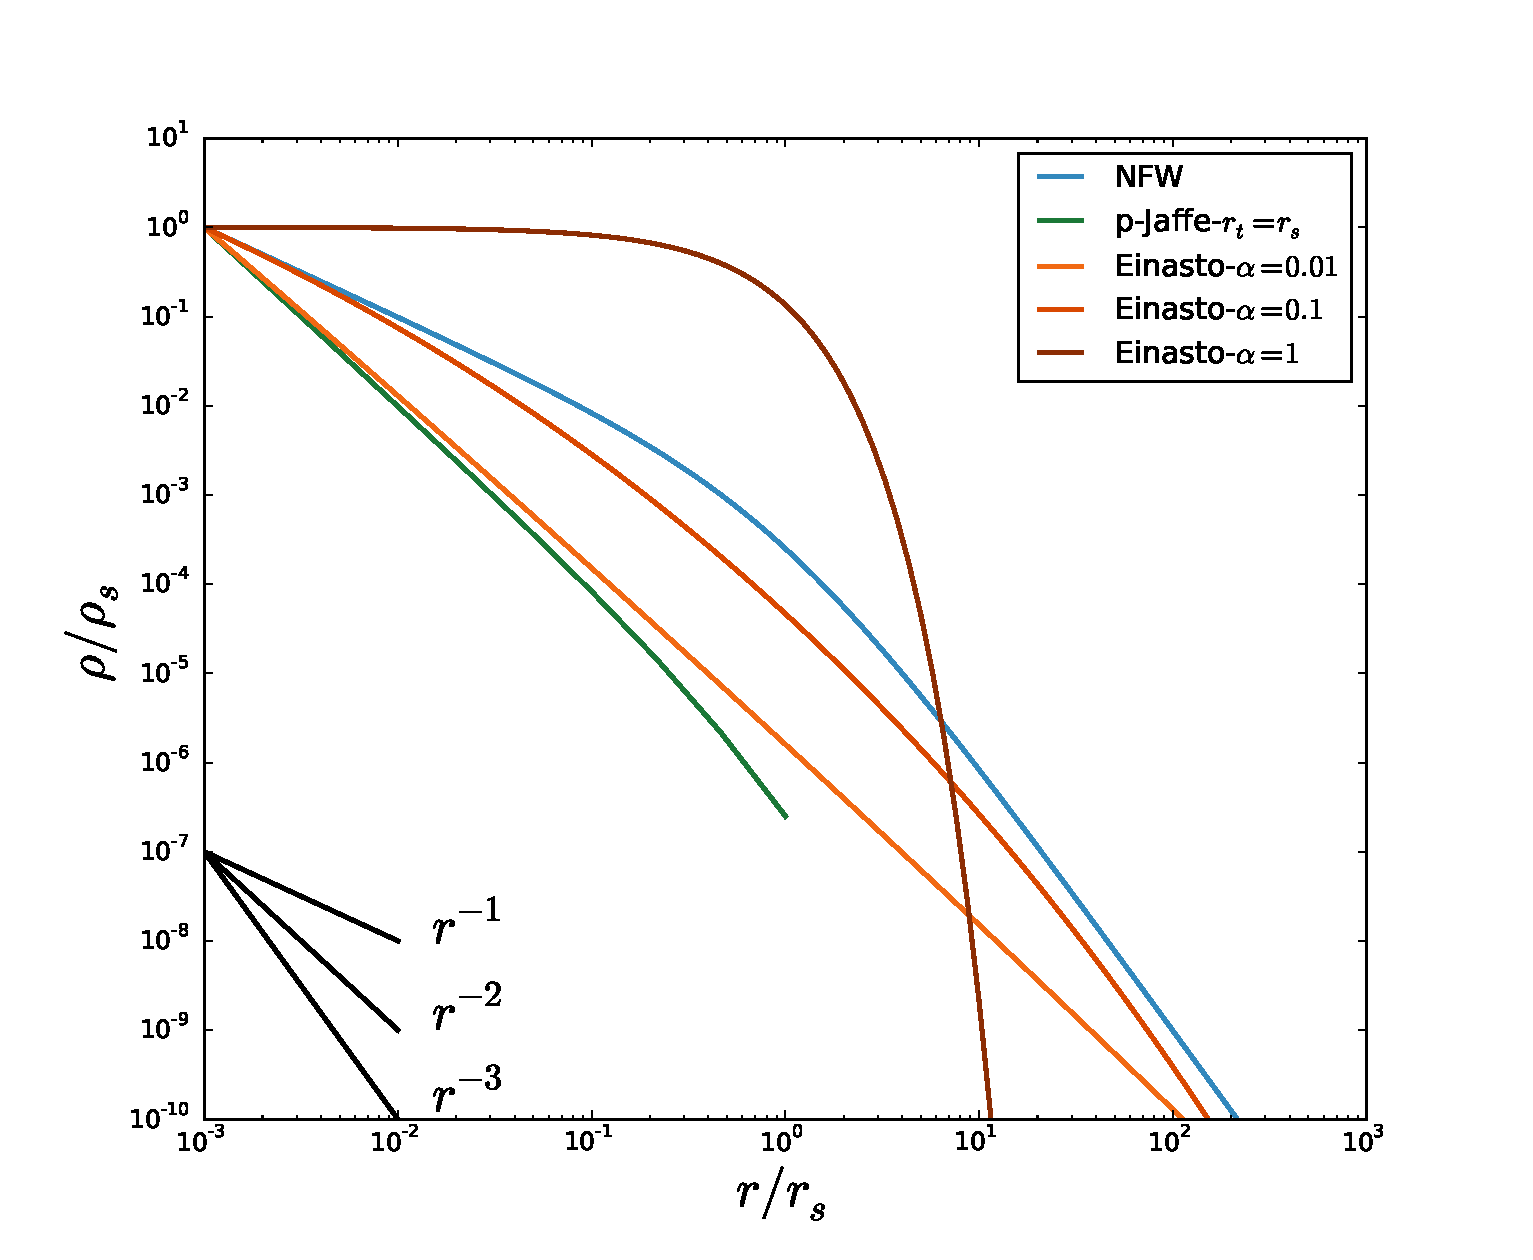
\includegraphics[width=0.5\textwidth]{figs/DensityProfiles}
%% \caption{Three different inner density profiles of dark matter halos; pseudo-Jaffe profile in green, the standard CDM halo profile suggested by NFW in blue, and the three--parameter Einasto profile with different Einasto indices in shades of brown. Three density slopes proportional to $r^{-1}$, $r^{-2}$, $r^{-3}$ are shown for comparison, where $\rho \propto r^{-1}$ corresponds to the central regions of the NFW profile, $\rho \propto r^{-2}$ to the isothermal profile, and $\rho \propto r^{-3}$ to the outer radii of the standard NFW profile.}
%% \end{SCfigure}

%\subsubsection*{Classical CDM subhalos (NFW)}
%\label{NFW}
%At $z=0$, the CDM scenario predicts the existence of dark matter halos with masses ranging from $\sim 10^{15}\ M_\odot$ down to the cutoff in the density fluctuation spectrum, which is set by the detailed properties of the CDM particles. For many types of WIMPs, this cut--off lies somewhere in the range $\sim 10^{-11}$--$10^{-3} M_\odot$ \cite{Bringmann2009}. However, alternative models involving superweakly interacting particles (superWIMPS) and MeV mass dark matter may place the cutoff as high as $\sim 10^3$--$10^8 \ M_\odot$ \cite{Hisano+,Hooper+}. 

%As these low--mass halos merge to form more massive ones, some temporarily survive in the form of subhalos within the larger halos. N--body simulations indicate that the subhalos within a galaxy--sized CDM halo should follow a mass function of the type:
%\begin{equation}
%\frac{\mathrm{d}N}{\mathrm{d}M_\mathrm{sub}}\propto M_\mathrm{sub}^{-\alpha},
%\label{subhalo mass function}
%\end{equation}
%with $\alpha\approx 1.9$ \cite{Springel+2008,Gao2008}. The relative contribution from subhalos with mass $M\gtrsim 10^5\ M_\odot$ to the dark matter surface mass density at the typical location of macroimages in a galaxy--mass lens is $f_\mathrm{sub}\approx 0.002$ \cite{Xu+2009}, albeit with a large scatter \cite{Chen+}. 


%where $R_\mathrm{S}$ is the characteristic scale radius of the halo. The slope of the inner density cusp ($\beta = \mathrm{d}\ln \rho /\mathrm{d}\ln r $) in this profile is $\beta = -1$, and this makes it difficult for NFW halos in the dwarf--galaxy mass range to produce millilensing effects of the type we are considering in this paper. Typically, cusp slopes obeying $\beta\lesssim -1.5$ would be required \cite{Zackrisson.Riehm2010}. Later work has shown that models with inner cusp slopes that become progressively shallower towards the center provide even better fits to isolated halos in CDM simulations, eventually reaching inner slopes of $\beta \geq -1$ \cite[e.g.][]{Navarro+2010}. In the context of detecting millilensing effects from low--mass halos, this just makes matters worse, since the central density is reduced.

%Traditional universal NFW profile for dark matter halos, is a 2--parameter model which describes the mass--density of the halo by the its mass, and concentration parameter. The halo concentration parameter is defined as $c \equiv r_{vir}/r_s$, where $r_s$ is the scale radius (the radius at which $\rho \propto 1/r^2$). The mass and concentration parameter are correlated, through a shallow slope. Besides, concentration parameter also is correlated with redshift. The is, however, not a single recipe for the detailed dependencies (see Bullock et al. 2011, others? for different opinions!). 

%Once a halo falls into the potential well of a larger halo and becomes a subhalo, it is stripped of material -- primarily from its outskirts -- due to interactions with its host halo and with other subhalos. This alters the density profile of the subhalo compared to an isolated halo of the same mass \cite[e.g.][]{Hayashi+,Kazantzidis+}, but these modifications tend to diminish rather than enhance the ability of a CDM subhalo to produce detectable millilensing effects \cite{Zackrisson.Riehm2010}. 

%To demonstrate that standard CDM subhalos do not provide a significant ``background'' of millilensing events in the observational situation that we consider, we have therefore adopted NFW profiles for these objects, since this results in an overoptimistic estimate on the millilensing effects that standard CDM subhalos are likely to produce. Even then, the chances of detecting millilensing effects from these objects turn out to be negligible in the observational situations we are considering. 

%To derive the $R_\mathrm{S}$ values of our NFW subhalo profiles, we adopt the mass--dependent concentration parameters $c=R_\mathrm{vir}/R_\mathrm{S}$ from either \cite{Bullock+2001} or \cite{Maccio+1998}, where $R_\mathrm{vir}$ is the virial radius of the halo. Since both of these recipes predict higher concentration parameters for low--mass halos, and since more centrally concentrated profiles (i.e. profiles with higher $c$) are more efficient in producing millilensing effects, we calculate the subhalo concentration parameters based on their current masses rather than the masses they had prior to becoming subhalos. Since nearly all subhalos have lost considerable amounts of material \cite[e.g.][]{Vale-Ostriker}, this also results in overly optimistic millilensing properties. 

%\subsubsection*{Three--parameter halo profiles (gNFW and Einasto)}
%The more general variation of the NFW profile, gNFW relaxes the central logarithmic slope $\gamma$
%\begin{equation}
%\rho(r) = \frac{\rho_s}{(r / r_s)^\gamma(a + r/r_s)^{3-\gamma}},
%\end{equation}
%where $\gamma = 1$ gives the traditional NFW profile and $\gamma = 2$ is equivalent to a singular isothermal sphere (SIS).
%Another 3--parameter profile is the Einasto profile, the tree dimensional version of the Sersic profile for surface brightness of elliptical galaxies \citep[][]{Einasto1965}. There are various studies confirming that CDM halos are better described by the Einasto profile, than the NFW one \citep[e.g. ] {Navarro+2004, Gao+2008, DiCintio+2014, Dutton.Maccio2014}. The extra parameter describing dark halo density profiles is the shape index, $\alpha$, which gives the density profile more flexibility in shape, i.e. $\gamma(r) = -dln\rho/dlnr \simeq 1/r$. 

%Both high-resolution measurements of central stellar and gas content of low surface brightness dwarf galaxies, and high--resolution CDM simulations, tend to indicate more consistency with a three--parameter density profile rather than the traditional NFW ones. }

%Navarro et al. 2004 found the Einasto index for halos in the mass range between dwarves and clusters is between 0.12 and 0.22, with an average value of 0.17. According to Hayashi \& White 2008 and Gao et al. 2008, $\alpha_E$ tends to increase with mass and redshift in halos of the Millennium simulation (Springer et al. 2005). From gravitational lensing point of view, Einasto profiles are more demanding to work with as for general $\alpha_E$ values, there is no analytical form for the surface mass density of these halos. Therefore, the lens equation needs to be solved numerically each time.

%However, Einasto profile still fails to describe observed dark matter halos inhabiting baryonic matter.   

%\subsubsection*{Halo concentration parameter $c$}
%Halo concentration is another parameter, in addition to the inner density slope that takes part in telling different halo models apart. The halo concentration parameter is defined as $c \equiv r_{vir}/r_s$, where $r_s$ is the scale radius (the radius at which $\rho \propto 1/r^2$). Halo virial radius as a function of redshift is calculated by ({Bullock et al. 2001}), while the concentration parameter follows a relation proposed by ({Maccio et al. 2007}).

%A cosmologically--motivated halo density profile is
%\begin{equation}
%\rho(r) = \frac{\rho_0 r_s^3}{(r_c + r)(r_s + r)^2},
%\end{equation}
%where $\rho_0$ is a characteristic halo density, $r_s$ is a scale radius (the radius at which $\rho \propto 1/r^2$), and $r_c$ is the core radius. 

%\subsubsection*{Maximum circular velocity $V_{max}$ and that of the infall epoch $V_{infall}$}
%\subsubsection*{Mass accretion history (MAH)}

\subsubsection{Normalization (The too--big--to--fail problem)}
\label{subsec:too-big-to-fail}
A more recent issue with the predictions of the cold dark matter model was brought up only a few years ago, pointing out another discrepancy in the structural properties of DM subhalos of MW--like simulated halos and dSph satellite galaxies of the MW. While one would naively expect that the most luminous dwarf galaxies correspond to the most massive subhalos, high--resolution cosmological simulations persistently produce massive subhalos ($M_{vir} \geq 10^{10} M_\odot$) which are too concentrated in their central kpc to host any of the satellite galaxies around the Milky Way or Andromeda. (\cite{Boylan-Kolchin+2011, Boylan--Kolchin+2012}). The combination of measured effective (half--light) radius $R_e$ and velocity dispersion $\sigma$ of a dSph with simple dynamical arguments can constrain the total mass of the dwarf within $R_e$. The Upper mass limits derived for the 8 most massive satellites of the MW, (excluding the Magellanic clouds), are systematically smaller than those of the 10 most massive subhalos in high--resolution cosmological simulations, within the same radii. Therefore, the most massive subhalos cannot host the most luminous dSphs of the MW. Consequently, unless MW halo is a very peculiar system, the most massive subhalos of the galaxy remain dark while the most luminous dSphs reside in intermidiate--mass dark matter halos, leave the least massive subhalos dark (corresponding to the overabundence of luminous satellites of the MW with $M_{300} \simeq 10^7 M_\odot$ reported by \citet[][]{Kroupa+2010}). One suggested explanation for this mismatch is that the halo of the MW is less massive than previously estimated and therefore, the local massive dSphs should be compared to simulated subhalos of a less--massive halo \citep[][]{Boylan--Kolchin+2012, Wang+2012, Vera--Ciro+2013}. However, a similar discrepancy has been observed within the local group \citep[][]{Kirby+2014, Garrison--Kimmel+2014, Tollerud+2014}, and even field galaxies \citep[][]{Papastergis+2015} as well, which argues for a more global issue, in need of a more generic solution. 

%Another proposed solution to the too--big--to--fail (TBTF) problem is that one should be cautious about the infall redshift of the halos when make an analogous between the luminosity function of dSphs and the mass function of their inhabit dark halos \citep[][]{}. 

%While the issue with the absence of density cusps in the center of faint galaxies, and the abundence of faint galaxies in the local Universe could be resolved by increasing the particle resolution of cosmological simuations and better adoption of baryonic feedback mechanisms, the too--big--to--fail (TBTF) issue is harder to explain. 



% However, ``the simplest formulation of the TBTF problem is as following: the mean densities inferred within the central few--hundred pc of the most luminous dSphs are systematically smaller than predicted in CDM simulation.'' Therefore, the problem is pointing to a more fundamental difference in simulated CDM halos and dSphs than the uncertainty in the MW halo mass.


\subsubsection{Spatial distribution (The satellite--planes problem)}
The issue with the spatial distribution of satellite galaxies of the MW was first argued to be challenging for the $\Lambda$CDM by \citet[][]{Ktoupa+2005}. Even though the spatial distribution of the [then] 11 satellite dwarves of the MW was not a new discovery, the fact that this alignment proposes a challenge to the stardar model of cosmology was new and in line with the rest of the small--scale issues proposed for this model. Upon the discovery of faint and ultra faint satellites of our galaxy in the SDSS survey, the presence of the satellite plane around the MW was confirmed \citep[][]{Metz+2009, Kroupa+2010}. The bonus argument made by \citet[][]{Metz+2009} uses not only the spartial distribution of dwarf satellites, but also their proper motions which is indicative of the majority of their sample orbiting within the vast plane of satellites (VPoS). A later work by \citet[][]{Pawlowski+2013} also confirms these results based on the proper motion measurements. The first question coming to mind in such a situation is about the locality of the observations. This question is adressed by various works ever since, both in the context of the [satellite and field] dwarf galaxies in our local group \citep[see e.g. ][]{Ibata+2013, Pawlowski+2013, Bellazzini+2013, Pawlowski.McGaugh2014a} and around more distant galaxies \citep[see e.g. ][]{Tully+2015, Muller+2015}. Even though the narrow dwarf galaxy plane of the MW is a widely--accepted feature in the data, the ubiquity of such planes in the rest of the Universe is under debate and needs further observational data with velocity measurements of satellite pairs in order confirm (or reject) them co--orbiting the host galaxy \citet[for opposite views on the matter see e.g. ][]{Phillips+2015, Cautun+2015}.


%\subsection{Separate problems or a systematic challenge?}
%\label{subsec:issues or systematic challenge}
%%{\bf Some of these mechanisms include inefficient cooling of atomic and molecular gas in halos of virial temperature $T_{vir} \leq 10^4$ K and $M_{vir} \leq 10^8 M_\odot$ \citep[e.g. ][]{}, loss of baryons to tidal and ram--pressure stripping and/or to photo--evaporation induced by cosmic reionization \citep[e.g. ][]{}, and inefficient accretion of baryons due to supersonic relative velocity between baryons and dark matter shortly after recombination \citep[e.g. ][]{}. However, consensus has not been reache on whether these mechanisms will cause sufficient loss of baryons in dark matter halos to hold responsinble for the absence of dwarf galaxies \citep[see e.g. ][arguing that there is more DM loss in tidal stripping processes than there is baryon loss]{Bullock+2010}.}
%%Whatever the particular mechanism is, the star formation efficiency needs to be less than ``normal'' in low--mass CDM halos.
%One major concern is the fact all these problems with the CDM paradigm arise on the same scale. (See ({Penarrubia et al. 2012}))

%Collisionless dark matter simulations, do not contain baryons and therefore the most massive subhalos in these simulations are assumed to be associated to the most luminous satellites. DM subhalo mass function is divergent on the low--mass scale, meaning for a consistent abundance match between satellite galaxies and DM subhalos, a strong suppression of star formation in low--mass (i.e. $M<10^{10} M_\odot$) subhalos is required. 
%The abundance of collapsed CDM subhalos increase exponentially toward small scales as $dn/dM_{vir} \propto M_{vir}^{-1.9}$.

%%\subsubsection*{The ``missing satellite'' and ``core/cusp'' problems}
%N--body simulations including pure $\Lambda$CDM, assume the gravitational interaction between WIMPs to be dominating the structure formation. As a result, one would expect galaxies to form within dark matter halos distributed in a mass function of the form $dn/dM_{vir} \propto M_{vir}^{-1.9}$ (Springel et al. 2008). Moreover, these halos form in a universal density profile centrally diverging as $\rho \propto r^{-1}$ , while the logarithmic slope decreases in larger radii, i.e. $\rho \propto r^{-3}$ for $r>r_s$ ({Navarro et al. 1996}). While central regions of normal galaxies are dominated by baryons, dwarf and low--surface--brightness galaxies show flat mass--density profiles in the center ({Oh et al. 2011}). 

% as well as a much flatter mass function than the one predicted by the simulations ({Klypin+1999, Moore+1999}). Either non--CDM models or non--gravitational interactions (like DM annihilation and such?) suggest solutions to these problems. However, there is not yet a single prescription resolving both discrepancies simultaneously. One proposed solution to the core/cusp problem lies in supernova gas flows, transferring energy to the dark matter component and flattening central density profiles. There are a number of proposed solutions to the suppression of galaxy formation in low--mass halos, e.g. ``SN feedback, inefficient cooling of ISM, cosmic reionization, UV radiation, and acoustic oscillations'' (e.g. Tassis et al. 2008, Bovill \& Riccotti 2009, Sawala et al. 2010, Bovy \& Dvorkin 2012). However, non has been successful to mark the discrepancy solved, moreover, the provided explanations do not work in coupling the missing satellite problem to the core--cusp issue. According to their model, ``the (minimum) star formation efficiency required to form DM cores in dSphs leads to an over--abundance of luminous satellites!''. Finally they conclude that the high--z core--formation cannot actually resolves the tension of opposite demands on star--formation efficiency \emph{on the same mass scales}, but only shifts it to lower luminosities.

%The problem arises when no M(total halo mass)--L relation can be found in the faint--end of galaxy luminosity function from observations of ultrafaint dSphs. Two possible explanations: The physical one is that the scatter in L at fixed $V_{max}$ is very large and is due to ``photoionization or suppression below the atomic cooling limit''. In other words (my interpretation), the total baryonic content is so low that once a small population of stars form within the halo they photoionize the rest of the baryons and there is not enough matter for efficient cooling (there only exists atomic cooling processes which doesn't offer sufficient cooling for the star formation cycle to continue), therefore, even though the halo is quite massive, the luminosity remain really low. The other possible explanation, on the other hand, is the product of a selection bias, as ``most ultrafaint galaxies inhabit halos with $M_{300}\leq 10^7 M_\odot$, but they are too diffused to have been discovered.'' 
%CONCLUSIONS AND DISCUSSION ro bekhun! (Bullock et al. 2010)

%DISCUSSION ro bekhoon!(Penarrubia et al. 2012)
%({Penarrubia et al. 2012}) make an estimate of the amount of energy required for cusp removal in the case of two massive MW dwarf spheroidal with relatively large observed cores (the dark halo core extends well--beyond the luminous radius of the dwarf!). They rule out the NFW profile for the halos of these galaxies with high confidence levels. They show that to reconstruct the observed large cores in thesw dwarf spheriodals from the cuspy DM profiles of the same $M_{vir}$, $\sim 10^{53} -- 10^{55}$ erg energy is required. Assuming the SNeII as the unique sorce of exerting such amount of kinematic energy to the gas in the central kpc of the dwarf, the model requires either (i) very efficient (close to $100\%$) SNeII energy transfer (into kinetic energy of the gas). This value, however, would be in disagreement with the relation between metallicity and luminosity of dSphs which suggests a value of $\sim 0.5\%$ instead (Governato et al. 2010) (ii) star--formation history peaking at very high redshifts (z$\geq$6) (why??) (iii) a very top--heavy IMF, therefore large number of SNe with less efficiency in energy transfer, (iv) ``substantial satellite disruption or other stochastic effects to ease the substructure abundance constraints'' (what??), otherwise keeps the low--mass end of galaxy mass functions cuspy. These small galaxies lack enough star formation, therefore SN--driven gas flow is insignificant. However, this requires high star formation efficiency in dwarf spheroidals with $M_{vir} \leq 10^{10}M_\odot$ (for them to show ``cored'' density profiles), while the missing satellite problem (flatter observed galaxy mass function than the predicted halo mass function diverging with $dn/dM_{vir} \propto M_{vir}^{-1.9}$ at the low--mass end),  strong suppression of star formation in order for these low--mass halos (on the same mass--scale) to remain dark (Penarrubia et al. 2012). They also argue that cusps must be removed in very high redshifts ($z > 6$) which is inconsistent with stellar ages of the two studied MW dSphs.

%In 2010, Bullock et al. wrote a paper on a potentially large population of low--luminosity dwarf galaxies within the halo of the MW. They argue that in case we impose a halo low--mass limit to the galaxy formation, only a handful of such dwarfs are expected in the halo of the galaxy. On the other hand, in the absence of such threshold in galaxy formation, the presence of these dwarfs, which are only different from the known ultrafaint dwarf galaxies is their slightly less--massive DM halos, implies that our common mass scale for MW dwarfs is merely an artifact of selection bias. 

%Halos 2013 -- White_1
%Issues:\\
%1) Inner density profiles; NFW or the bulk of mass -- Central cusps (nature of DM)\\
%SPH simulations by Zolotov et al. (2012) suggest dynamics associated with star formation may flatten cores in more massive dwarfs\\
%2) Shapes as predicted: shapes from lensing (individual clusters or stacked galaxies) -- Orbits of the streams in the MW or M31 halos\\
%3) Substructure as predicted: Effects on disks? GCs? Streams? -- {\bf Effects on strongly lensed BG object} -- Satellite counts; abundances, $M_*$ vs. $V_{max}$ relations\\
%Gaps in the Pal5 star stream (at $> 99\%$ confidence) may be induced by $> 1000$ substructures within 30 kpc with $V_{max} > 1$ km/s, consistent with $\Lambda$CDM predictions, discussed in Carlberg, Grillmair $\&$ Hetherington 2013\\
%4) Correspondence of halo/subhalos to galaxies\\
%Galaxies form by cooling and condensation of gas in halo cores, they are associated with subhalos, not halos. Not all subhalos may have a galaxy. Not all galaxies may have a subhalo in a DM--only simulation -- Springel et al. (2001)\\
%Subhalo abundance matching is sensitive to numerical resolution (Guo $\&$ White 2013)\\
%%Halos 2013 -- Navarro_10
%CDM halos are formed inside--out.\\
%Substructure contributes less than $\sim 10\%$ of the total mass.\\
%CDM halo substructure appear to be self--similar. i.e. halos of different mass, properly scales, look alike.\\
%The --scaled-- subhalo mass function is independent of the host halo mass (Zheng et al. 2005 -- Lravtsov et al. 2004)\\
%Typically, halos have only one subhalo more massive than $\sim 3\%$ of the host halo Virial mass. (Wang et al. 2012)\\
%Only 3 MW satellites appear to inhabit halos more massive than $V_{max} \sim 30$ km/s, while --on average-- 10 subhalos more massive than this are present in Aquarius halos (Boylan--Kolchin et al. 2012)\\
%The spatial distribution of subhalos is independent of halo mass. Most subhalos populate the outer regions os the halo.\\
%The shape of the mass profile of the DM halos is roughly independent of halo mass and cosmological parameters.\\
%Density profiles are {\bf cuspy} and clearly differ from power laws.\\
%Usually parameterized by a mass, $M_{200}$, and concentration, $c \equiv r_{200}/r_s$\\
%Models to predict the mass and redshift dependence of the concentration (eg. Bullokc et al 2001, Eke et al 2001, Neto et al 2007, Gao et al. 2008)\\
%%Recent analysis indicates a puzzling upturn in the concentration of rare, massive halos, which is clearly inconsistent with a formation redshift interpretn for the concentration. (Prada et al. 2010)\\
%The mass profile of CDM halos deviates slightly but systematically from universality in very high--resolution simulations. Therefore, a third parameter seems needed to describe the mass profile in detail, as in the Einasto profile ($\alpha = 0.17$ resembles the NFW profile). (Navarro et al. 2004)\\
%Based on the Millennium simulations: The concentration depends systematically but {\bf weakly} on halo mass. This relation, and its dependence on redshift have proved very difficult to reproduce. Models that use the halo accretion history rather than a formation redshift seem to work best (Wechsler 2002, Zhao et al. 2003). At a given mass, average halos are NFS--like, outliers are not. (Ludlow et al. 2013)\\
%The origin of the concentration and shape parameters: The concentration measures the characteristic density of a halo ans is assumed to trace the formation redshift of the halo, although the definition of the latter has been unclear! Mass profile and accretion history are closely related (Lu et al. 2006, Wu et al. 2013)\\
%The shape of the mass profile resembles that of the accretion history. Both are well approximated by the NFW shape. Similarity of mass profiles is due to similarity of mass accretion histories. \\
%Generally, there is good agreement between the mass profiles of galaxy clusters and those of CDM simulations. Only some tension remains regarding the concentration of strong--lensing clusters AND the slope of the inner density cusp. The slightly higher concentration of strong--lensing clusters is thought to reflect projection effects of highly aspherical clusters.\\
%%One thing I'm gonna need to remember is the regime where strong lensing can meaningfully probe density profiles. I think this rather famous plot is for galaxy clusters but it shows that it's only in a range between 10 and 100 kpc that multiple images technique is a good probe for the density profile. For smaller radii, kinematics dominate and for the larger radii, weak lensing is what's probing the density profile. I do not know why, especially when there is no baryons... (Newman et al. 2013)
%cusp vs. core problems highlights for dwarf galaxies remain inconclusive. Do we really need baryons to modify substantially the dark matter halo??\\

%%Halos 2013 -- Koopmans_2
%Dark matter on scales of $< 1$ kpc: Is there CDM substructure? Methods: flux ratio and surface brightness anomalies
%In a galaxy--galaxy lensing system, the Einstein radius of the system is much larger than can be explained by stars alone for any reasonable IMF, lens or dynamical model.

%Dark matter on scales of 1--10 kpc: What is the DM fraction inside $R_{eff}$, $R_{Ein}$?
%How is DM distributed (slope/concentration)?
%Can DM explained by dark stars? IMF??

%DM on scales of 10--100 kpc: Extended DM halos through combined strong and weak lensing

%What's not matching is the luminosity function of galaxies in the dwarf galaxy mass range to to mass function of dark matter halos as predicted by N--body simulations
 
%%	Ludlow et al. 2013	%%
%%%%%%%%%%%%%%%%%%%%%%%%%%%%%%%%%%

%Proposed methods to detect such substructures around th eMW rely on gamma--ray emission from the annihilation of dark matter, or on the gravitational scattering of stars in the tidal streams of satellite galaxies.\\
%There is this new method proposed by Feldmann \& Spoylar on 2013, based on the substructures gravitational pull on stars of the MW disk.\\
%The number density of dark matter halos encodes invaluable information about the primordial power spectrum, the physics of early universe and the nature of dark matter. (Moore+1999, Bullock.Kravtsov.Weinberg 2000, Kuhlen+2012)\\
%in WDM models, a competitor of the CDM paradigm, structure formation is suppressed below the free--streaming scale of the dark matter particle, resulting in a deficit in substructure with masses below $\sim 10^9 M_\odot$ (Zentner \& Bullock 2003)\\


%%%%%%%%%%%%%%%%%%%%%%%%%%%%%%%%%%%%%%
%A spatially unresolved measurement of the flux density from a lensed source is a factor of order $\mu$ brighter than for an unlensed source, while spatially resolved measurements can provide a factor of $\sqrt(\mu)$ higher resolution. (Schneider et al. 1992)

%----------------------------------------------------------------------------------------

\newpage
\section{Gravitational Lensing} 
\label{sec:Gravitational lensing}
The deflection of light is a predictable phenomenon in the framework of Newtonian mechanics, serving as one of the major tests of general relativity by the famous 1919 solar eclipse experiment \citep[][]{Eddington+1919}. In Newtonian description, light photons are treated as test particles being influenced by gravity of a massive object. Therefore, a test particle passing with velocity $v$ near a point-like massive object, $M$, with an impact parameter $\xi$, is deflected by an angle $\alpha$. Considering a very small deflection angle (the most likely case in cosmology), $\alpha$ is given by

\begin{eqnarray}
\label{eq:alpha}
\alpha \simeq \frac{4GM}{v^2 \xi}.
\end{eqnarray}

In the case of a light beam, where $v = c$, passing very close to the surface of the Sun, the deflection angle turns out to be $\sim$ 0.85 arcseonds. This value coincides with what was obtained by Einstein prior to the final formulation of GR, provided space is considered Euclidean not affected by gravity of the Sun. However, the pre-relativistic predicted deflection angle is half the predicted angle by general relativity in its fully developed form. The factor added by general relativity represents the local spatial curvature produced by the mass and was proven to be consistent with observational results in 1919 for the first time. Several groups measured the angular shift of stars projected close to the solar limb during a total eclipse \citet{Eddington+1919}. This served as the second evidence in support of GR, after perihelion precession of Mercury. Based on the calculation using the generalization of this phenomenon for two distant stars, it was generally accepted that the separated images of a star due to the gravity of another star was impossible to detect with the technology of the day. A few years later, Fritz Zwicky suggested  \citep{Zwicky1937} that the effect of an extragalactic ``nebula'', i.e. a galaxy, rather than a foreground star is big enough and should have been observed by then. Even though his calculation was too optimistic due to overestimating the masses of galaxies at that time, the idea of utilizing this phenomenon as a ``natural telescope''  remained as a curiosity until 1979 when for the first time two identical quasars ($0957+561$ A \& B) were revealed in an observation \citep{Walsh+1979}. The similarity of the spectra of the two quasars with the same redshifts, $z \sim 1.41$, and 6 arcseconds angular separation were mostly accepted to be convincing evidence for the fact that the two objects are physically associated. Furthermore, finding a galaxy at a lower redshift close to the two images lent more support to the idea that this was another case of gravitational lensing. Several cases of gravitational lensing have been found and investigated ever since.

\subsection{Mathematical Description}
Here I strat with setting up the gemoetrical framework for the gravitational lensing assuming a point--like lens (the same calculations for an extended lens requires integrating over the projected lens area). Another simplifying factor is the ``thin lens approximation'', implying that the impact parameter of the lens is considerably small compared to the distances in the system, thus the extension of the lens along the line of sight is ignored.

The relation between the unlensed source position, $\boldsymbol \beta$, and the position of the image(s), $\boldsymbol \theta$, is called the \emph{lens equation}. This equation can be derived geometrically from the setup displayed in figure \ref{fig:config} and shown below:

\begin{eqnarray}
\label{eq:lens_eq_angle}
\boldsymbol \beta = \boldsymbol \theta - \frac{D_{ds}}{D_s} \hat{\boldsymbol \alpha}(\boldsymbol \xi).
\end{eqnarray}

 where the image position is $\boldsymbol \theta = \frac{\boldsymbol \xi}{D_{d}}$. Hence, by substituting $\alpha$ with the expression found in equation \ref{eq:alpha}, we have

 \begin{eqnarray}
 \label{eq:lens_equation}
 \boldsymbol \beta = \boldsymbol \theta - \frac{D_{ds}}{D_s D_d} \frac{4GM}{c^2 \boldsymbol \theta}.
 \end{eqnarray}

 Alternatively, using the distance from the source to the optical axis, in the source plane,  $\boldsymbol \eta = D_{s} \boldsymbol \beta$, the lens equation becomes

\begin{eqnarray}
\label{eq:lens_eq_distance}
\boldsymbol \eta = \frac{D_s}{D_d}\boldsymbol \xi - D_{ds}\hat{\boldsymbol \alpha}(\boldsymbol \xi)
\end{eqnarray}

\begin{figure}[][t]
 \label{fig:config}
 \centering
%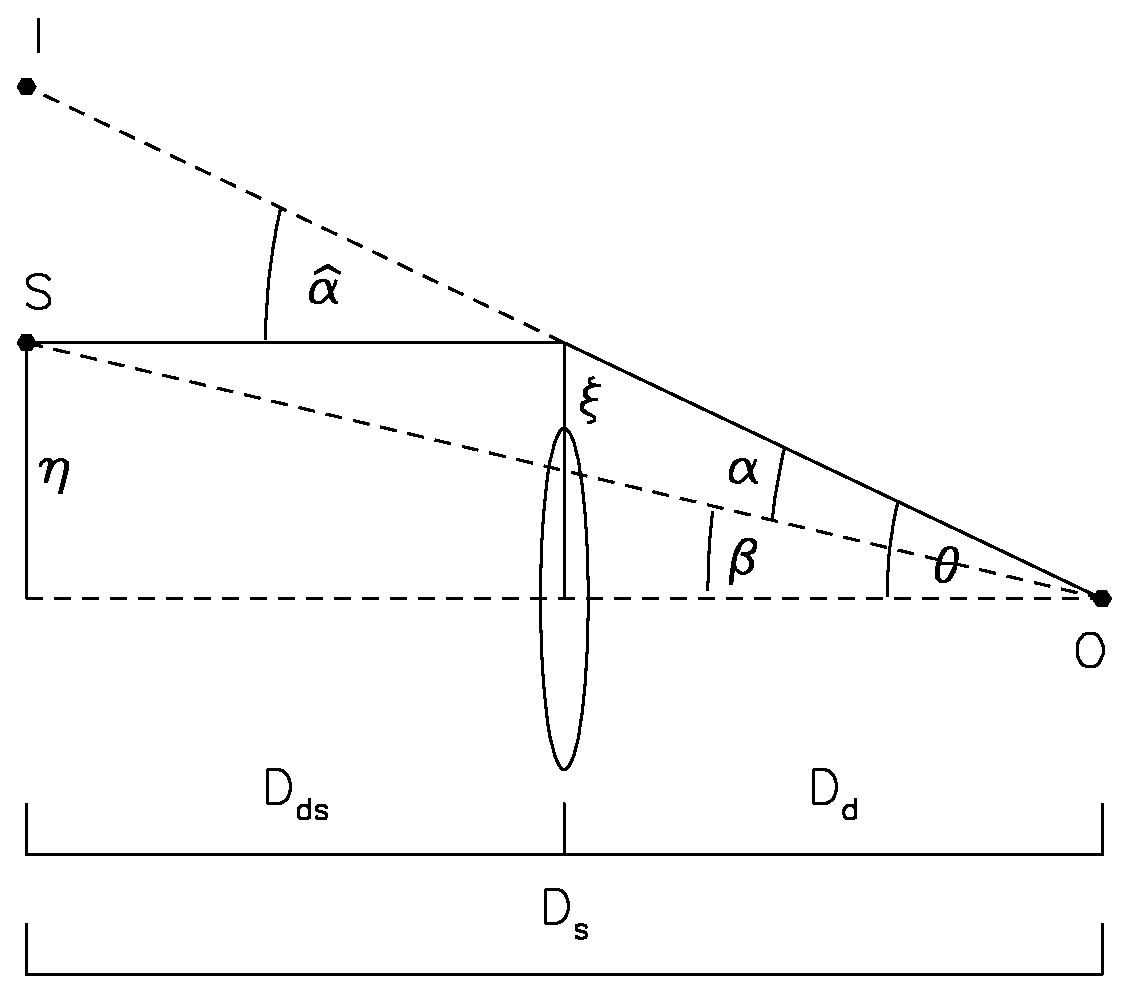
\includegraphics[width=0.5\textwidth]{figs/setup}
% \caption{The relation between angles and distances in a gravitational lensing setup as described by the lens equation. In this schematic figure, $O$ represents the position of the observer, $S$ is the source and the lens (deflector) is reduced to its projection on a plane perpendicular to the line of sight, as assumed in the ``thin lens approximation''. (Figure adopted from \citet{narayan_lectures_97}).}
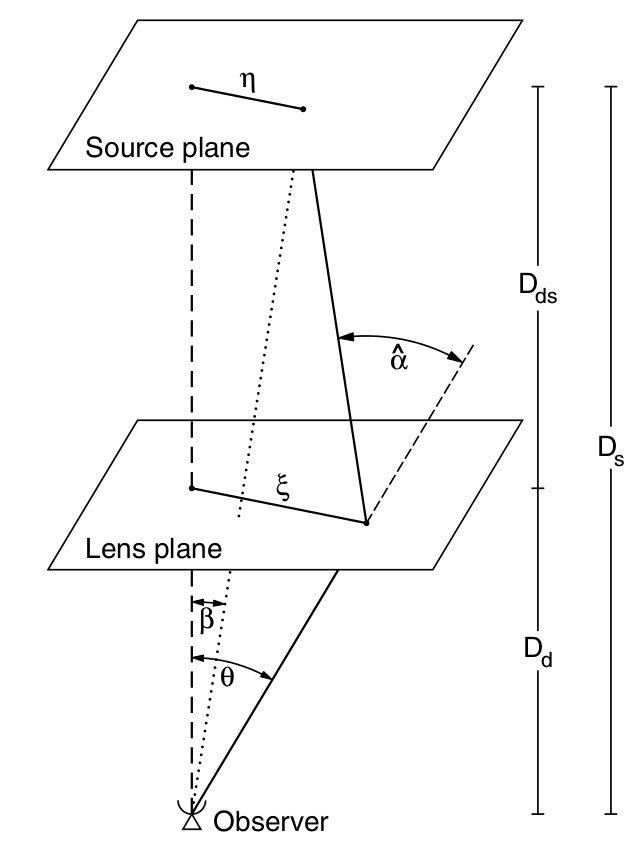
\includegraphics[width=0.5\textwidth]{figs/Gravitational-lensing-angles}
 \caption{The relation between angles and distances in a gravitational lensing setup as described by the lens equation. In this schematic figure, $O$ represents the position of the observer, $S$ is the source and the lens (deflector) is reduced to its projection on a plane perpendicular to the line of sight, as assumed in the ``thin lens approximation''. (Figure from Wikipedia}
 \end{figure}

Given a certain mass distribution and a fixed $\boldsymbol \xi$, the lens equation can have more than one solutions for $\boldsymbol \theta$; each of which corresponds to an image of the source in the sky.  Although obtaining the source position $\eta$ from a given image position $\xi$ using the lens equation is straightforward, finding a general analytical solution for the position of the image(s) of a source at a given position is not. Keeping in mind that the mapping of $\xi$ to $\eta$ is non--linear. There are, however, analytical models to solve this equation for simple matter distributions on the lens plane such as point--mass, axially symmetric, and elliptical lenses.

The deflection angle due to the surface mass density of the lens gives rise to a deflection potential $\psi$ of the form $\boldsymbol \alpha = \nabla \psi$. Accordingly, another way of presenting the lens equation is in the form of 

\begin{eqnarray}
\label{eq:potential_dimensionless_lensing}
\textbf{y} = \nabla \left(\frac{1}{2}\textbf{x}^2 - \psi(\textbf{x}) \right)
\end{eqnarray}

where $\textbf{x} \equiv \frac{\boldsymbol \xi}{\xi_0}$ and $\textbf{y} \equiv \frac{\boldsymbol \eta}{\eta_0}$ are dimensionless vectors, when $\xi_0$ and $\eta_0$ are length scales in the lens plane and the source plane, respectively. This form of expressing the lens equation leads to the formulation of Fermat's principle in gravitational lensing theory

\begin{eqnarray}
\nabla \phi(\textbf{x}, \textbf{y}) = 0
\end{eqnarray}

where $\phi$ is a scalar function as below

\begin{eqnarray}
\phi(\textbf{x}, \textbf{y}) = \frac{1}{2} (\textbf{x} - \textbf{y})^2 - \psi(\textbf{x})
\end{eqnarray}

Fermat's principle states that the light ray always chooses the path which takes the least \emph{time} to pass through. Therefore, it can be used to relate the time delay between two separate images of a single source to the considered cosmology and mass distribution of the lens.


Light deflection is a propagation phenomenon, influencing only the shape of the light bundle from the source, and not the surface brightness {\bf ref. on surface brightness conservation when dealing with multiple images}. Therefore, for a monochromatic source, we have the received flux from the source as 

\begin{eqnarray}
S = I_{\nu} d\omega
\end{eqnarray}

where $d\omega$ is the differential solid angle, and $I_{\nu}$ is the monochromatic surface brightness. Since $I_{\nu}$ is not affected by gravitational deflection, the flux changes are merely mirrored in solid angle variation of the image. Hence, the \emph{magnification} due to gravitational lensing is defined as the solid angle ratio of the observed image to that of the non--lensed source

\begin{eqnarray}
\label{eq:mu_domegas}
|\mu| \equiv \frac{d\omega}{d\omega_0}
\end{eqnarray}

On the other hand, the solid angle is related to the angular position of the image (source), via the dimensionless quantities \textbf{x} (\textbf{y}). Therefore, the magnification due to a circularly symmetric lens is given by 

\begin{eqnarray}
\label{eq:mu_beta_theta}
|\mu| = \frac{\theta d\theta}{\beta d\beta}.
\end{eqnarray}

One of the most interesting and extreme cases of gravitational lensing is the Einstein ring. The lensing setup which gives rise to a complete Einstein ring consists of a point--like source, with a spherically symmetric lens, both of which are collinear with the observer, i.e. the lens is centered around the line of sight between the observer and the source. Therefore, the observer sees a ring--shaped image with an angular radius of $\theta_E$ which is called the angular Einstein radius. This radius, $\theta_E$ is obtained by substituting $\beta=0$ in equation \ref{eq:lens_equation} as:

 \begin{eqnarray}
 \theta_E = \sqrt{\frac{4GM}{c^2}\frac{D_{LS}}{D_LD_S}}.
 \label{eq:lens}
 \end{eqnarray}

 Where $M$ represents the lens mass and $D_L$, $D_S$, and $D_\mathrm{LS}$ are the angular--diameter distances as in figure \ref{fig:config}. Moreover, as it is immediately concluded from equation \ref{eq:mu_beta_theta}, magnification $\mu$ diverges for the \emph{critical points} where $\beta=0$. The ``infinite'' theoretical magnification ({\bf explain why infinite magnification is only a theoretical concept}) points can be mapped into the source plane which gives a set of \emph{caustic curves}. The number and relative positions of images of a single source change according to the position of the source with respect to such caustics in the source plane. (see figure \hyperref[fig:cusps]{2.2}).

 \begin{figure}[ht]
 \label{fig:cusps}
 \centering
 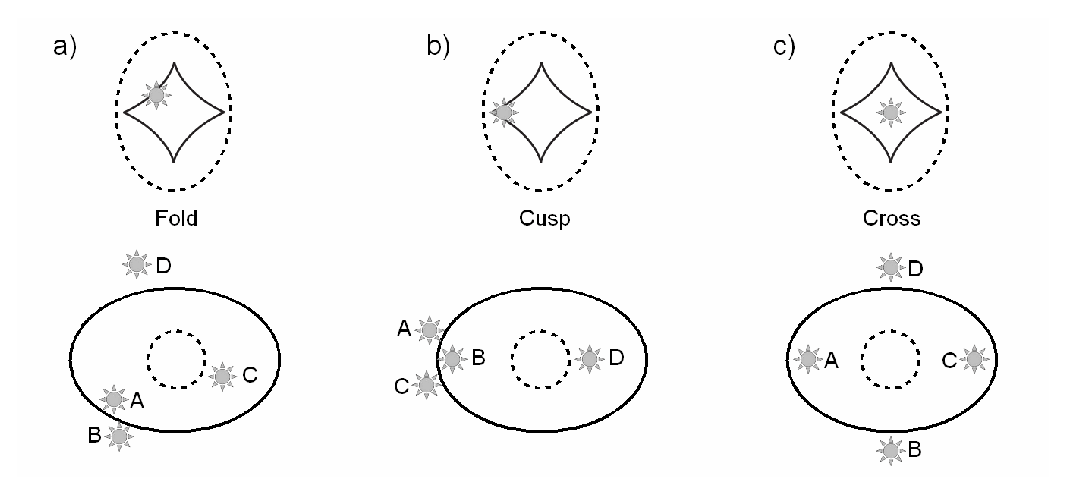
\includegraphics[width=1.0\textwidth]{figs/zack09_4}
 \caption{Different configurations of a four-image lens: a) Fold, b) Cusp and c) Cross. The upper row shows the caustics and position of the source (star) in the source plane. The solid line indicates the inner caustic and the dashed line the outer caustic. A source positioned inside the inner caustic produces five images. A source positioned between the inner and outer caustic produces three images, whereas a source positioned outside the outer caustic will not be multiply imaged. In the case of multiple images, one of the images is usually highly de-magnified, so that only four- and two-image lens systems are observed, respectively. The lower row shows the corresponding critical lines and resulting observable images in the lens plane. The inner caustic maps on the outer critical line and vice versa. A close pair (A, B) and a close triplet (A, B, C) are produced in the fold (a) and cusp (b) configurations, respectively. (Figure and caption adopted from \citet{Zackrisson.Riehm2010})}
 \end{figure} 

 \subsection{Strong and Weak Lensing}
One observable result of gravitational lensing is magnified (or de-magnified) images of point sources, the other distortions in the images of extended objects. The extent of the lensing effect varies depending on the alignment of the source, the lens and the observer. The closer the center of the lens to the line of sight between the observer and the source, the more significant the image distortion. Therefore, gravitational lensing cases are categorized, according to the level of their magnifications, into two major regimes; \emph{strong} and \emph{weak} lensing. Strong lensing causes dramatic effects such as high magnifications, multiple images, luminous arcs and in some cases even complete Einstein rings. Although strong lensing is a rare effect, it is possible to be detected and studied individually for each case. Weak lensing, on the other hand, occurs when the center of the lens is further away from the observer's line of sight, i.e. $\theta > \theta_E$. Thus the images are weakly magnified or have small distortions. In contrast to strong lensing, weak lensing happens to be very common. Every line of sight is affected by weak lensing at some level hence this effect is detectable through statistical investigations of numerous objects. 

\subsubsection{Strong Lensing}
As pointed out in the previous section, the lens equation (equation \ref{eq:lens_equation}) can have multiple solutions. Moreover, when the ``thin lens approximation'' is valid, the surface mass density of the lens, i.e. the projected mass of the lens on the lens plane, determines the severity of the gravitational lensing case. Accordingly, one can introduce the constant \emph{critical surface mass density} $\Sigma_{\mathrm{crit}}$ such that for every $\theta$ in the lens equation \ref{eq:lens_equation}, we have $\beta = 0$.

\begin{eqnarray}
\label{eq:Sigma_crit}
 \Sigma_c &=& \frac{c^2}{4 \pi G}\frac{D_{os}}{D_{ol} D_{ls}}.
\end{eqnarray}

In cases where $\Sigma > \Sigma_{\mathrm{crit}}$, multiple images from the background source are produced. Exceeding the critical surface mass density may happen only for a part of a specific foreground galaxy or galaxy cluster, the solid angle of which is then called the \emph{strong lensing cross section}. 

On the other hand, the magnification of the image due to the presence of the lens which was defined by equation \ref{eq:mu_domegas}, can also be expressed with the following relation 

 \begin{eqnarray}
 \label{eq:mu_kappa_gamma}
 \mu = \frac{1}{(1 - \kappa)^2 - |\vec{\gamma}|^2}
 \end{eqnarray}

 which is obtained by substituting the determinant of the Jacobian matrix for the lens equation. In this form, there are two quantities upon which the magnification is dependent, \emph{convergence} $\kappa$ and \emph{shear} vector $\vec{\gamma}$. Convergence, which describes the local isotropic magnification of the source, is a scalar quantity and is defined as the surface mass density of the lens in the unit of the critical surface density as below

 \begin{eqnarray}
 \label{eq:convergence}
 \kappa &\equiv& \frac{\Sigma}{\Sigma_{\mathrm{crit}}}
 \end{eqnarray}

 Shear is the measurement of the distortion of the source image and is quantified along each position component on the lens plane, thus a vector. The magnification for point sources is a tensor, only dependent on $\kappa$ and $\vec{\gamma}$, however, for an extended source it is more complicated, depending on the internal surface brightness distribution of the source.

\begin{SCfigure}
  \centering
  \label{fig:shear_convergence}
  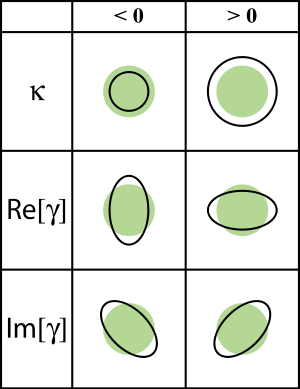
\includegraphics[width=0.3\columnwidth]{figs/shear_convergence}
  \caption{from Wikipedia} %https://en.wikipedia.org/wiki/Gravitational_lensing_formalism
\end{SCfigure}

   \subsubsection{Strong Lensing Regime}
Strong lensing cases are studied within sub--regimes differing by the angular separation of multiple images produced by each. The angular separation of gravitational lens systems producing multiple images is typically of the order of the Einstein radius of the lens $\theta_E$. Accordingly, the terminology used for various strong lensing separations is

\begin{itemize} 
\item \emph{Macrolensing} refers to cases with typical angular separations, Einstein radii, of the order of \emph{arcseconds}. Macrolensing can be thought as the combined effect of the dark and luminous matter of an isolated galaxy as well as the effect of galaxy clusters or multiple galaxies along the line of sight. 
\item \emph{Millilensing} (sometimes called \emph{mesolensing}) effects, may be produced by satellite galaxies or their dark counterparts, dark matter subhalos, as well as small--scale objects such as intermediate--mass black holes (IMBHs), with typical multiple image separations in the order of \emph{milliarcseconds}. Therefore, lensing effects in this regime potentially address one of the small--scale issues of the CDM theory, the so--called "missing satellites problem" which is mainly the subject of chapter \ref{chap:missing_satellite_problem}. However, the compound effects due to this phenomenon could be in a much larger regime, depending on the mass function and spatial distribution of these substructures \citet{Treu10}.
\item \emph{Microlensing} refers to Einstein radii of solar-- and planetary--mass lenses, i.e. the order of \emph{microarcseconds}. Unlike macrolensing and millilensing, microlensing is a transient effect such that it is observable through monitoring a source for a period of time and recording its light curve. The apparent brightness of the source varies over time as the alignment of the lens system changes due to the moving lens. This type of gravitational lensing is not considered in the present study.
\end{itemize}

Following the same convention, strong gravitational lensing cases with smaller angular separations are referred to as nanolensing ($\theta_E \sim 10^{-9}$ arcseconds), picolensing ($\theta_E \sim 10^{-12}$ arcseconds), femtolensing ($\theta_E \sim 10^{-15}$ arcseconds), etc. However, the terms above are what I mainly use in this thesis.

 \subsubsection{Astrometric Perturbation}
 The proximity of the projected image of a foreground massive object to a background source has effects on various angular scales. Among many, one is a change in the apparent position of the source. This effect which is usually accompanied by magnification or distortion effects is called the \emph{astrometric effect}. Astrometric effects are, therefore, detectable mostly in dynamic cases, such as microlensing cases, where the observer can actually follow the temporal differences in the relative positions in the system. One of these cases stems from the presence of substructures in the main lens such that where the deflector consists of a parent halo with a distribution of subhalos inside. 
 
  When it comes to the astrometric perturbation due to the substructure inside a halo, the macroimage gets shifted from its original position, under the influence of the subhalo. This effect is mostly sensitive to intermediate and high mass substructures \citet{Moustakas+2009} and in clearly visible in the results of the present work (see figure \hyperref[fig:astrometric_perturbation]{2.3}).

 \begin{figure}
\label{fig:astrometric_perturbation}
\centering
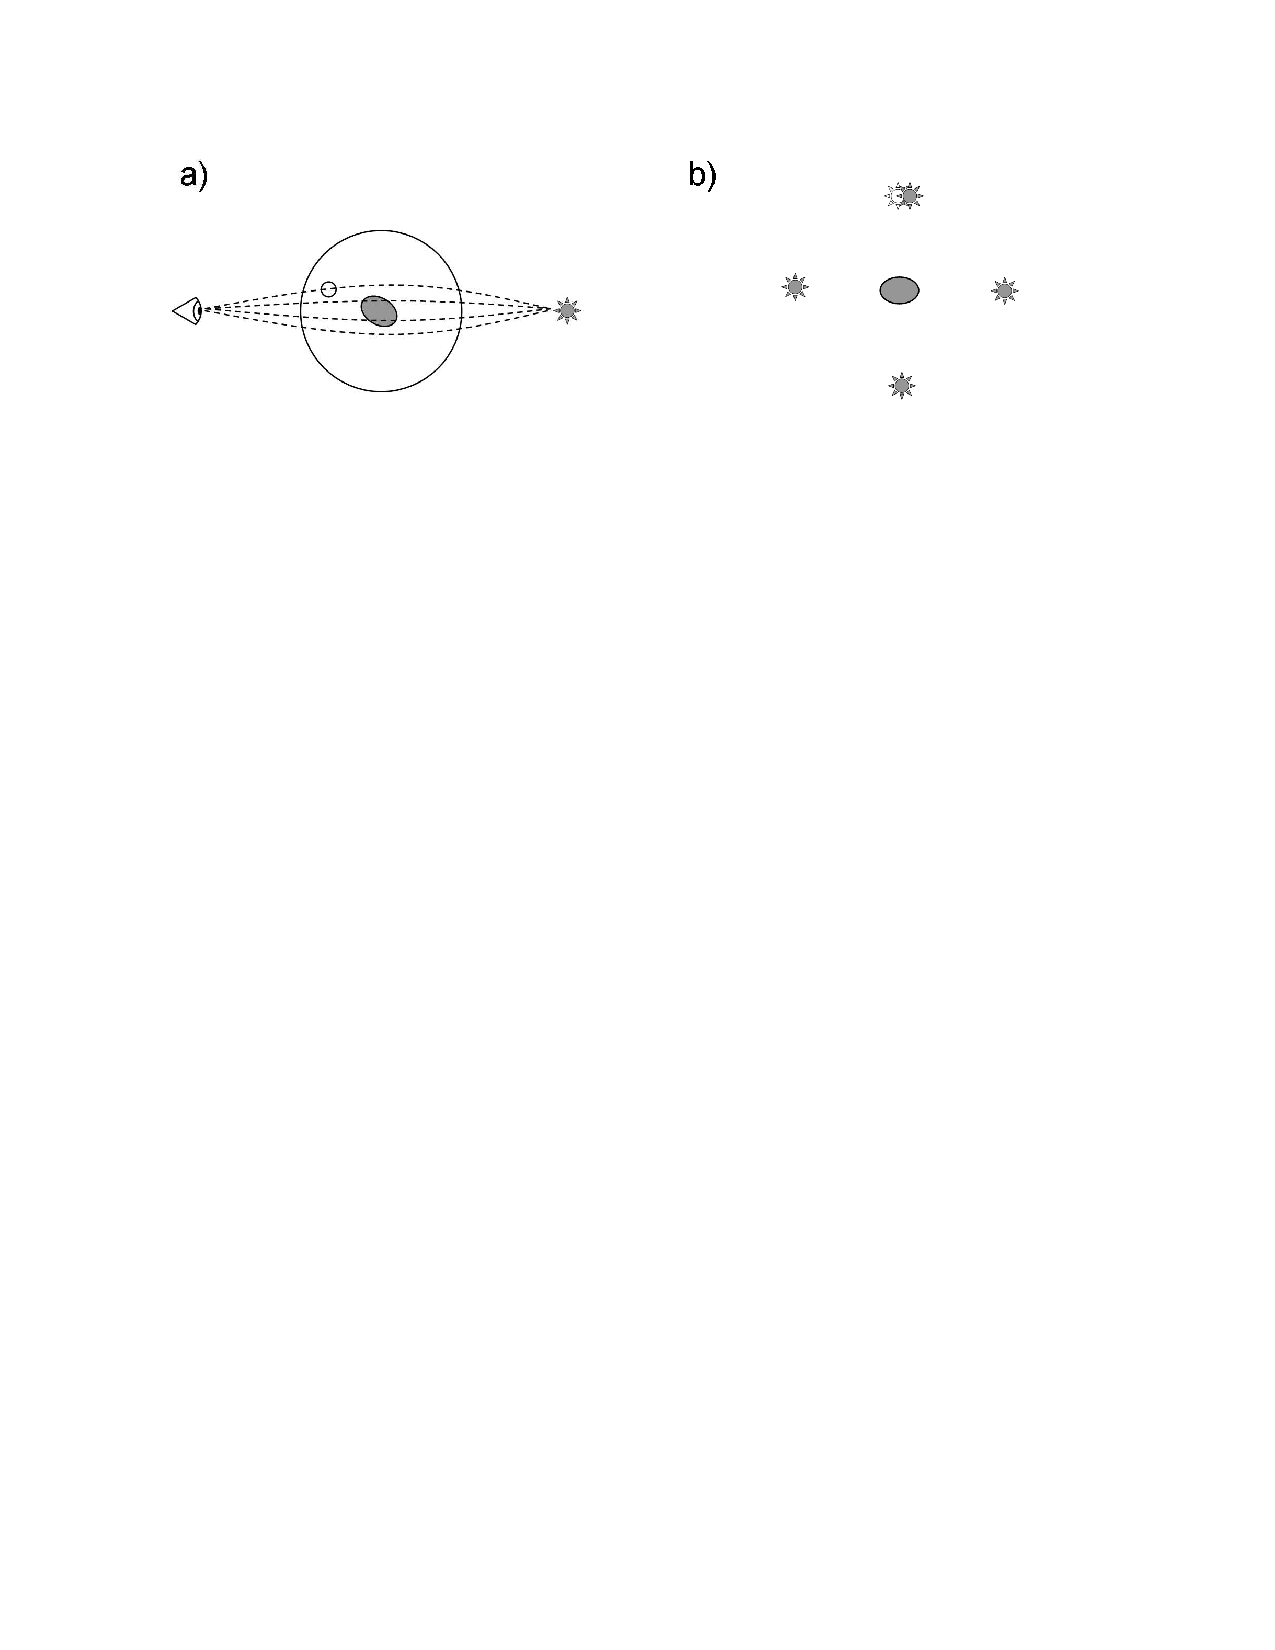
\includegraphics[width=1.0\textwidth]{figs/astrometric_perturbation}
\caption {Astrometric perturbations. a) One of the multiple sightlines towards a distant light source passes through a dark subhalo. b) The images of the macro--lensed source are observed at the positions of the gray source symbols. Modeling of the lens system with a smooth lens potential predicts the position of the upper image at the white source symbol. The subhalo close to the sightline of the image causes a deflection on the order of a few tens of milliarcseconds. (Figure and caption adopted from \citet{Zackrisson.Riehm2010})}
 \end{figure}
 
 \subsubsection{Time Delay}
 Each macroimage follows a different path to reach the observer, i.e. is subject to a different time delay. This time delay consists of two independent components; the geometrical and the gravitational component. The geometrical term comes from the difference in the light path length for each image. The gravitational component, also known as the \emph{Shapiro} effect, is a relativistic effect of retardation in strong gravitational fields. However, different time delays of various images cannot be observed if the source is not intrinsically variable, since this effect is manifested in the phase difference of the light curves of various images. When it comes to subhalo hunting, the perturbation to the time delays between macroimages predicted by a smooth lens model serves as an evidence for the presence of substructures within the main lens (see figure \hyperref[fig:time_delay]{2.4}). As \citet{Moustakas+2009} argue, such an effect is only sensitive to subhalos at the high--mass end of the mass function.
 
 \begin{figure}[h]
 \label{fig:time_delay}
 \centering
 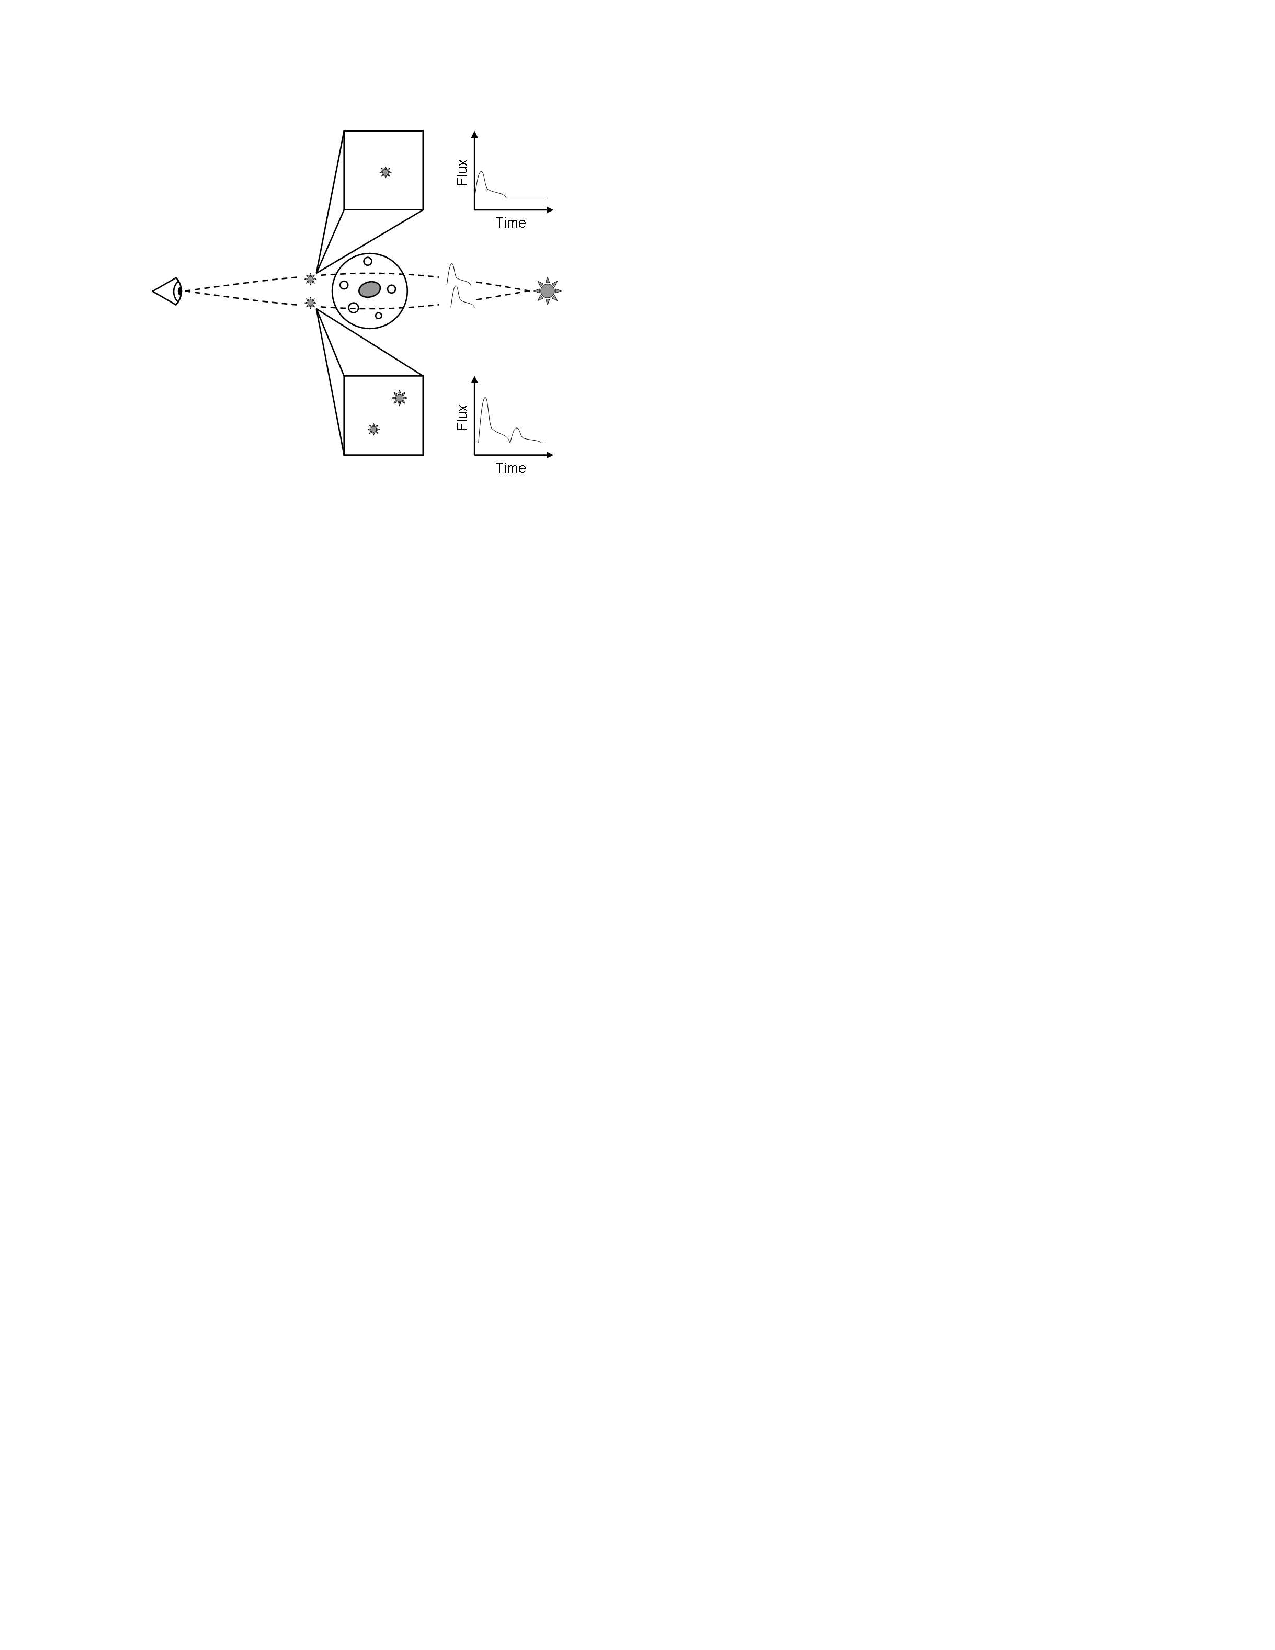
\includegraphics[width=0.5\textwidth]{figs/time_delay}
 \caption{A galaxy with a dark matter halo produces distinct macroimages of a background light source. If this source dis-- plays intrinsic variability, observable time delays between the different macroimages may occur. If one of the macroimages experiences further small--scale image splitting due to a sub-- halo along the line of sight, a light echo may be observable in the affected macroimage. This may serve as a signature of millilensing in cases where the small--scale images blend into one due to insufficient angular resolution of the observations. (Figure and caption adopted from \cite{Zackrisson.Riehm2010})}
 \end{figure}
 
 {\bf Time delay is the only gravitational lensing observables that changes with the length scale of the lensing setup.} Given two lensing setups merely differing in angular--diameter distances, the only variable which breaks the degeneracy of the observables is time delays of various images.
 
 \subsubsection{Flux Ratio Anomalies}
 \label{subsec:Flux Ratio Anomalies}
Gravitational lensing is a propagation phenomenon, thus it conserves the number of photons. On the other hand, the gravitational deflection influences the cross section of the light bundle differentially. Consequently, in order to conserve the flux, the area of the image(s) of the source changes. This leads to different magnifications for different macroimages, as explained in equation \ref{eq:mu_domegas}. However, mere determination of the flux of a single image does not provide any information if the intrinsic flux of the source is unknown. The observable quantities, are rather the flux ratio and positions of two separate macroimages of a single source.

%----------------------------------------------------------------------------------------

\newpage
\section{Radio interferometry}
In this section, I briefly explain the main principles based upon which radio interferometers work. I, also, try to put radio interferometry into the context of radio astronomy as well as observational astronomy, in general.

%\subsection{Basic hardware and electronics of radio telescopes}
\subsection{Radio telescopes}
A radio telescope is usually made of two main parts:
\begin{itemize}
\item Reflector: The special shape of this reflector, i.e. a parabola, is advantageous compared to convex mirrors used in reflecting optical telescopes as the parabolic shape keeps all reflected radiation  in phase and as I will repeatedly mention in this section, coherence is of great importance in radio astronomy. Keeping the same principle in mind, current radio instruments use aperture arrays keeping the electromagnetic wave coherent at the receiver by exerting appropriate delays to the signal.
\item Receiver: Unlike optical telescopes which scan different points of the focal plain with numerous receivers (pixels of a CCD), radio telescopes generally work with a single receiver at the focal point of their reflector. In other words, radio telescopes see the entire sky within a single pixel only!

Heterodyne receivers are the most common kind of receivers used in radio antennae today, and although in principle they could be arranged in 2--D arrays on the focal plane of the antenna to perform as a CCD in an optical system, the cross--talk among closely placed receivers makes the calibration of each receiver cumbersome and usually inefficient. A more practical approach would be to use several parabolic reflectors (aperture arrays) simultaneously to observe several pointing on the sky.
\end{itemize}
Heterodyne receivers are the most common type of receivers at sub--mm wavelengths (and higher) and they are crucial to use if the signal modulation (both amplitude and phase of the signal) is needed for observations (the case in radio interferometers)\\
%{\bf I do not really know the difference between a heterodyne and a bolometric receiver but I need to write *briefly* about them}

In order to digitally record the electromagnetic wavefront reaching the receiver, the signal needs to be sampled with a frequency at least twice the frequency of the wave (Nyquist theorem). This is an electronically challenging task, and particularly impossible for frequencies in the order of 100 GHz and higher. Therefore, the arriving signal is first mixed with the signal from a stable local oscillator (LO) with a well--known frequency slightly lower than that of the original signal. The mixed signal then has two frequencies $f_\mathrm{sky} + f_\mathrm{LO}$ and $f_\mathrm{sky} - f_\mathrm{LO}$. Therefore, we can sample the low frequency signal with as fine resolution as desired, ignoring the higher frequency. The signal is then {\bf demixed} by exerting a phase difference and is recorded in two frequency windows below and above the LO frequency, namely the \emph{lower sideband} and the \emph{upper sideband}, by the receiver.

\subsection{Observational limitations}
Observational limitations of the recorded data may come from the source or, more commonly, from our instruments and can be classified into limitation in 
\begin{itemize}
\item resolution
\item sensitivity
\item dynamic range
\end{itemize}
As will be discussed further into the section, radio interferometry has brought significant improvements in the former two, although mostly at the cost of the latter.

\subsubsection*{The convolution theorem}
What a radio telescope records is not the direct image of the source at different points at the same time, a radio telescope rather records signals from the entire sky into a single ``pixel'' and so does an array of radio antennae. Radio interferometry is based on \emph{the convolution theorem}. According to this theorem, it can be shown that convolving two functions in Fourier space (i.e. Fourier transform of their convolution) is equivalent to multiplying the Fourier transform of the two in the ordinary space.
\begin{align} 
\begin{split}
\mathcal{F}(f*g) &= \mathcal{F}(f) \times \mathcal{F}(g)
\end{split}                    
\end{align}
Where convolution of one function $f(t)$ with another function $g(t)$ means shifting the function $g$ consecutively from $t=-\infty$ to $t=+\infty$, while at each step the multiplication of the two functions (i.e. $f(t)g(t+\tau)$) is added to the convolved function $f*g$:
\begin{align} 
\begin{split}
\mathcal (f*g)(\tau) &= \int_{-\infty}^{+\infty} f(t)g(t+\tau) dt
\end{split}                    
\end{align}
No device can achieve infinite resolution due to its diffraction limit, which results in spreading the light from a point source into its surrounding pixels, aka. point spread function (PSF) of the instrument. Therefore, anything observed with that instrument will be seen as the convolution of the true source structure with the PSF. Angular resolution of an instrument (i.e. FWHM of its PSF) scales with the size of the aperture and wavelength as $\Delta\theta \propto \lambda / D$. Therefore, the PSF itself scales with the square of the Fourier transform of the aperture which, according to the convolution theorem, equals the Fourier transform of the autocorrelation of the aperture. Therefore, in order to increase the resolving power of an instrument, one needs to either increase the aperture size or decrease the observing wavelength. While the former solution might not be possible to arbitrary large extent due to different physical emission mechanisms, the former is in the heart of using the interferometry technique.    
 
\subsection{Two-element interferometer}
When we talk about interferometry, clarification is needed to distinguish between the common picture of Young's optical double--slit interferometer and the concepts and techniques used in radio interferometers. In the optical case, the fringe pattern made on the detector plane is a distribution of points with various intensities $I(x) = |E_1(x) + E_2(x)|^2$, and visibility is a real quantity between 0 and 1 defined as below:
\begin{align} 
\begin{split}
V &= \frac{I_\mathrm{max} - I_\mathrm{min}}{I_\mathrm{max} + I_\mathrm{min}}
\end{split}                    
\end{align}
Visibility in the case of radio interferometry, however, is a complex quantity describing the time correlation of the two signals reaching the two elements of the interferometer and can be expressed as below:
\begin{align} 
\begin{split}
\label{eq:vis_def}
V(\tau) &= <E_1(t)E_2^*(t+\tau)>
\end{split}                    
\end{align}
with $\tau$ being the geometrical time delay between the two signals due to the different paths the wave needs to reach each antenna.
\begin{align} 
\begin{split}
\tau &= \frac{\vec{B}.\vec{S}}{c}
\end{split}                    
\end{align}
Where $\vec{B}$ is the three-dimensional distance vector between the two elements, aka. \emph{baseline}, $\vec{S}$ is the source vector and $c$ is the speed of light.

Practically, the time delay $\tau$ of one signal with respect to the other is added to the signal electronically to correct for this effect before sending the two signals to the correlator. Applying the geometrical time delay $\tau$ is equivalent to projecting the baseline connecting the two telescopes on the plane perpendicular to the direction of the source. Therefore, what matters in all math hereafter is the \emph{projected} baseline between the two antenna, rather than the actual baseline. 

The correlated signal is a complex visibility describing the response of the interferometer to the two signals, both amplitude and phase, received from a point source which is a fringe pattern (on the sky) perpendicular to the projected baseline ($BL_\mathrm{proj}$) as seen from that point on the sky. What happens in radio interferometry is that we sample the visibility values on this plane depending on the position of the source, $BL_\mathrm{proj}$, and duration of observations. The interferometer's response to an extended source is simply the superposition of the response patterns of various point sources making up the extended source. In other words, the measured visibility is the integral of source structure multiplied by the response. Therefore,
\begin{align} 
\begin{split}
V_\mathrm{observed} &= \int V^\text{point source}_\text{response} I(x, y) dx dy.
\end{split}                    
\end{align}
Where $x$ and $y$ are celestial coordinates and $I(x, y)$ is the intensity distribution of the extended source.

\subsubsection*{The van Cittert-Zernike theorem and the interferometer equation}
As long as the source we are observing is far enough that the wavefronts from the source can be approximated as plane waves (i.e. Fraunhofer approximation applies), the complex visibility of the source only depends on the relative position of the two observed points, and the wavelength the observations are made at. The visibility function, then, is a measure of the spatial coherence of the wavefront of the source encoding the source structure in it.
\begin{align} 
\begin{split}
\label{eq:vC-Z}
V^\mathrm{AB} = <E_A \times E_B^*> = \mathcal{F}(\frac{\vec{R_A} - \vec{R_B}}{\lambda})
\end{split}                    
\end{align}
The left hand side is, by definition, the complex visibility of the source, $\vec{R_A} - \vec{R_B}$ is the observing baseline, and $\mathcal{F}$ is the Fourier transform of the source structure $I(x, y)$. Therefore, rewriting the interferometer equation, one finds:
\begin{align} 
\begin{split}
\label{eq:InterferometerEq}
V(x,y,z) = \int_{x,y} I(x, y) e^{-\frac{-2\pi j}{\lambda}(ux+vy+wz)} \frac{dx dy}{z}
\end{split}                    
\end{align}
where $z=\sqrt{1-x^2-y^2}$. If x and y are small enough so that the observing field can be approximated as flat, the $wz$ term becomes zero and the mere geometrical delay correction means that both receivers are probing the same coherent wavefront. This interferometry equation transforms the intensities on the source plane to visibilities on the image plane and their values depend on the coordinates of the observing baseline, projected on the source plane, as well as the structure of the source and the observing frequency. 

\subsection{Aperture synthesis}
%\subsection{Multi-element interferometers and aperture synthesis}
Back to the definition of visibility in radio interferometry, one can directly conclude that a multi--element interferometer is only a combination of several two--element interferometers, sampling the (u, v) space in pairs, based on their projected baseline and the observing frequency, measuring the visibility at those sample points only. 

\subsubsection*{Snapshot observations}
Fourier transform is blind to the absolute baseline position, but as baseline is a vector, it does carry information about the direction of the baseline. This implies that in a multi--element interferometer, a [arbitrary] frame of reference is needed for combining the antenna pairs and calculating the transformation from the ordinary plane to the (u, v) plane. The (u, v) coverage in a snapshot is equal to the autocorrelation of the array configuration as seen by the source -- except for the central point which corresponds to the measurement with the hypothetical $BL = 0$, impossible to implement in practice.

Since Fourier transform is a \emph{Hermitian} transformation, a single baseline corresponds to sampling not one, but two points on the visibility plane; one at (u, v), and the other at (-u, -v). Moreover, if I(x, y) is a real number, $V(u, v) = V^*(-u, -v)$. This means that each baseline gives two separate visibility measurements. This means that adding even one more antenna to the array has a significant effect on better sampling the (u, v) plane; One via increasing the number of baselines ($N_\mathrm{BL} = \frac{N_\mathrm{ant}(N_\mathrm{ant}-1)}{2}$), and the other, via double--sampling each baseline as mentioned above. Therefore, a monofrequency snapshot made by an interferometer with $N_\mathrm{ant}$ antennae makes $2N_\mathrm{BL}$ discrete visibility measurements where longer baselines in the (u, v) plane correspond to smaller scales on the image plane and vice--versa. Besides, as seen in equation \ref{eq:InterferometerEq}, the conversion between the (x, y) plane and (u, v) plane is scaled by the observing frequency. Therefore, a wider observing bandwidth would result in a wider radial coverage of the (u, v) plane. As (u, v) coordinates are measured in wavelength, one way of filling the Fourier space is to observe at multiple wavelengths simultaneously. The other way to upgrade the discrete sampling of (u, v) space , closer to a continuous sampling (in the tangential direction), is longer exposure time. In this mode, the Earth rotation would lead to a continuous change in projected baselines of the array as seen by the source and hence more (u, v) coverage.

Two extreme regions of the (u, v) plane are usually the most challenging to fill. Long baselines (corresponding to small scales on the image plane) are difficult to achieve for obvious practical reasons and therefore the longest baseline in the array sets the angular resolution of the reconstructed image and obviously the impossibility of infinite baselines make the infinite resolution also impossible! On the other hand, short spacings on the (u, v) plane could also be challenging to achieve because of the minimum spacing forced by antenna sizes. This leads to a fundamental feature of any (u, v) sampling known as ``zero-spacing hole''. The lack of visibility measurements on this scale corresponds to missing out on any possible (smooth) large-scale structure on the source such as diffused emission. In cases where an unrecovered diffused component does exist in the original source, the integrated flux of the source measured using the interferometer would be smaller than the integrated flux of the target measured by a single-dish telescope. This is a tell--tale signature of the presence of a large unrecovered structure in the source and is known as ``the missing flux'' problem. The problem arises due to the poor (or lack of) sampling the short spacings on the (u, v) plane. Therefore, the intensity profile of an internally Gaussian source, lacks data points in the center thus visibility interpolation tends to flatten out the peak. In many cases, sampling the short spacings with a more compact array or a single--dish telescope helps constrain a better fit to the light profile of the source.

\subsubsection*{Aperture synthesis and image reconstruction}
Aperture synthesis is the technique of reconstructing an image from incomplete sampling of the Fourier space. The technique is based on modeling the visibility plane based on the existing samplings. Therefore, the more complete the (u, v) coverage, the closer the model image to the real one seen by the antennae. However, there will always be holes in the sampled (u, v) plane limiting the fidelity and quality (i.e. $\text{dynamic range} = \frac{\text{peak}}{\text{RMS}}$ of the reconstructed image.)

Fourier transform of the (u, v) coverage gives the so-called ``dirty beam'' (equivalent to the point spread function PSF), while the Fourier transform of the measured visibilities on the (u, v) plane results in the ``dirty image'' of the source, which is, as expected, the actual source structure convolved with the dirty beam. Now that we have images of both the beam and the source, we can deconvolve the beam from the image. Remember that deconvolution is non-linear and non-unique! (See section \ref{sec:CLEAN} CLEAN algorithm)

Despite what it looks like, modeling is actually applied while working in the image plane. The process is such that the dirty beam and dirty image are calculated based on the (u, v) coverage and direct visibility measurements, respectively. For this purpose, the (u, v) plane is required to be gridded\footnote{In fact, this is the issue one faces when using \emph{Fast} Fourier transform (FFT), while \emph{direct} Fourier transform does not require griding the (u, v) plane. One would expect the resulting image to be nearly the same as the model obtained by natural weighting. However, direct FT is so much slower that it is not worth practicing as far as the visibilities are sampled wisely!}. At this step, Nyquist sampling of the (u, v) plane introduces a limitation in the image space, i.e. grid size/cell size needs to  be chosen such that the final PSF includes at least 3 pixels in the image plane. The next step in image reconstruction is deconvolving the beam from the dirty image. The actual interpolation happens here! Deconvolution is not a unique process, hence requires not only griding the (u, v) plane but also making assumptions about the deconvolving beam. One assumption need to be made is how to weight the measured visibilities. This question, in turn, has two parts: How are the measured visibilities in one (u, v) pixel weighted? and what is the relative weight of various pixels on the (u, v) plane? Different choices at this step result in different angular resolution and dynamic range limitations in the model image.

\paragraph*{Natural weighting} as it sounds is simply weighting visibilities inversely proportional to the variance of their distribution.
Therefore, short--spacings in the (u, v) plane , with closer samplings, are weighted more than longer baselines which results in higher dynamic range in the modeled image at the cost of a coarser angular resolution. In other words, the dirty beam has larger FWHM, but less prominent side lobes. Therefore, it is best for imaging faint and smooth sources.

\paragraph*{Uniform weighting} is the same as natural weighting with an additional factor inversely proportional to the number of visibilities in each pixel. Therefore, it boosts the contribution from long--spacings by giving the same weight to visibilities at all (u, v) distances, even though those at long distances are sampled more coarsely. This property makes this approach more suitable for sources with rich and complicated structure. Although, the source needs to be bright enough for this approach to work best. This is because, the described weighting scheme results in a narrow(er than naturally--weighted) PSF, with smaller side lobes and therefore, better angular resolution. However, the RMS of the residuals of this model tends to be large(r than that of natural by at least an order of $\sim 2$), i.e. poorer sensitivity.

\paragraph*{Briggs weighting} is a tunable combination of both approaches above. The tunability of Briggs' recipe is applied through the \emph{robust} parameter. This parameter changes in the range of -2 to +2 from uniform to natural weighting. Usually, robust=0.5 gives a good compromise between the two extreme approaches. Although it still depends on the preferences based on the scientific target.

\paragraph*{(u, v) tapering} is useful when the observed source is extended and most of the information lies in short baselines. Therefore, in order to improve the SNR, we can overweight the measurements made using these baselines even further and decrease the weight of measurements where we have a lower signal, i.e. long baselines. This can be done via Gaussian circular tapers in the (u, v) plane. If the source has a very extended structure, which is remained unrecovered due to the short--spacing hole in the (u, v) coverage, even with natural weighting, then (u, v) tapering is the last resort to recover that diffused emission. 

As a matter of fact, one might want to get rid of an extended emission they are not interested in, and focus more on the small--scale clumpy structure of their source. In which case, one only needs to apply an inverse Gaussian taper to the (u, v) plane.

The method used in {\bf paper II} \ref{paperII} is based on combining different weightings of the same measurement set to put emphasis on features with different angular scales. 
\subsubsection*{CLEAN algorithm and deconvolving the dirty beam}
\label{sec:CLEAN}
While interferometry data are incomplete due to lack of information on -- most of -- spatial frequencies, we can interpolate the (u, v) plane by applying our prior information about the source structure as the criteria required to proceed with deconvolution. Clearly, the more our prior information about the source, the more reliable the model image is.

The problem of deconvolving dirty beam from the dirty image has non--unique solutions. An intuitive way to show it is assuming a source with non--zero visibilities everywhere but where we are making our measurements, i.e. our (u, v) coverage. This class of sources remain invisible to the interferometer, as long as the (u, v) coverage is the same. Now, one can add \emph{any} combination of these ``invisible'' sources to our reconstructed image without the measurement set changing. Improving the (u, v) coverage will decrease the number of these combinations and therefore, increase the image fidelity, and yet \emph{high} fidelity is not the same as \emph{infinite} fidelity. Therefore, the reconstructed image always remains a model of our real data.
% I know that I have brought this up several times by now but this is in the heart of the subject and I cannot emphasize it too much!

CLEAN \citep[][]{Hogbom1974} is the oldest, fastest and best deconvolution algorithm practiced to day for image reconstruction in radio interferometry. Talking briefly (and naively), what this algorithm does is to start at the maximum flux point in the image, subtract the PSF at that point and add a 2-D Gaussian component (with the same FWHM of the PSF and scaled flux) to the CLEAN image instead then repeat these three steps for the peak in the residual map until either of the criteria below is met: 
\begin{itemize}
\item Noise limit: If the peak in the residual map has a smaller value than $\alpha \sigma_\mathrm{RMS}$ 
\item Dynamic range limit: If the peak in the residual map has a smaller value than $\frac{1}{\alpha} \times f_\mathrm{max}$. of the dirty beam
\\($\alpha$ is an arbitrary coefficient set by the scientific purpose of the image.)
\item Maximum number of CLEAN cycles, which is an experimental (arbitrary) criterion.
\end{itemize}

%no (statistically-significant- peak remains in the dirty image.

Finally, what the algorithm produces are three matrices below:
\paragraph*{CLEAN model:} A set of point sources subtracted from the dirty image, where flux peaks located.
\paragraph*{CLEAN beam:} The corresponding Gaussian to the dirty beam. In other words, the PSF model. If the dirty beam is elliptical, then the CLEAN beam is also a similarly--elliptical Gaussian.
\paragraph*{CLEAN image:} It is simply the CLEAN model convolved with the CLEAN beam and is the final product of the image reconstruction procedure. 


While different deconvolution algorithms apply different criteria to the source structure, the CLEAN algorithm's basic assumption is that the source is made of discrete Dirac delta functions, i.e. point sources. Therefore, it tends to convert smooth and diffused components into clumpy ones. While one does not loose real emission by not CLEANing it, it is possible to get artificial features by CLEAning noise!

%developed a variant of the Clark algorithm whereby the major cycle subtracts `CLEAN' components from the un-gridded visibility data. Aliasing noise and griding errors can thus be removed if the inverse Fourier transform of the `CLEAN' components to each u,v sample is accurate enough. Two routes are used for the inverse transform:

%    for small numbers of `CLEAN' components, a `direct Fourier transform' is performed so the accuracy is limited by the precision of the arithmetic;
%    for a large number of `CLEAN' components, an FFT is used for efficiency, but inevitably some errors are introduced in interpolating from the grid to each u,v sample. High order Lagrangian interpolation is generally used. 

The current commonly--used implementation of CLEAN is the Cotton--Schwab CLEAN, consisting two same--level, linked cycles.
% \emph{Major cycle}s, each looping over a number of \emph{Minor cycle}s as below:
Start with a {\bf Minor cycle} as below:
\begin{enumerate}
\item Locate the peak intensity in the dirty image.
\item\begin{enumerate}
    \item Subtract a dirty beam centering at the point of the peak, from the dirty image.
    \item Compute the residual image = image used in step (1) -- product of (2.a).
    \item Scale down the flux density in residual image to {\bf g} times the image peak, where {\bf g} is the arbitrary CLEAN gain value.
    \end{enumerate}
\item\begin{enumerate}
    \item Add a point--like component to the CLEAN model, at the position of the peak.
    \item Set the flux density of the point in CLEAN model to the peak of the PSF.
    \item Convolve the newly--added point of the CLEAN model with the CLEAN beam and add it to the CLEAN image
    \end{enumerate}
\item Use the product of step (2.b) in step (1). 
\end{enumerate}
A {\bf Major cycle}, then, follows the minor cycle as below:
\begin{enumerate}
\item Compute model visibilities corresponding to the CLEAN model made in the minor cycle.
\item Compute the residual visibilities = observed visibilities -- model visibilities made in step(1).
\item FFT the residual visibilities and feed it to the next minor cycle 
\end{enumerate}
%{\bf Q: Which one do we feed the minor cycle with? output of the major cycle or output of the previous minor one? If latter, why do we bother with the major cycle then??}\\

While the CLEANing process seems complete within the minor cycle, the major cycle is needed because the algorithm (minor cycle only) cannot subtract anything from marginal parts of the image, where we have no information about possible sources in those regions whose side lobes (only!) affect our dirty image.


%http://www.quantumdiaries.org/2013/06/26/does-dark-matter-really-exist/
%Einasto 2013 -- Profumo 2012 -- Popolo 2013 -- Profumo 2013

%----------------------------------------------------------------------------------------

\newpage
\section{Summary}
With the fast imrpovement of observational facilities, the required angular resolution and sensitivity for the discovery of comound lens systems increase. Given all the uncertainties in the existence, abundence, mass function, and inner mass distribution of dark matter substructure it is important to estimate the alignment probabilities of lens substructures combined with the detection limits. It is important to keep in mind that with a detailed picture of model expectations at hand, even null detections provide constraints on the background model.

In {\bf paper I}, we use simulations of strongly lensed quasar jets as observed by three different VLBI configurations and receivers to probe dark matter substructure. The dark matter substructure used in this paper is the very dense form of halo substructures (intermediate--mass black holes and ultracompact minihalos) within the main lens at $z \simeq 0.5$. The small--scale morphological distortions in one of the macroimages that is not replicated in others in a large number of macrolensed jet systems with the expected (submilliarcsecond) resolution of the array, is used to set constraints on detection limits of such substructres and their abundence. We argue that intermediate--mass black holes with $M_\mathrm{IMBH} \sim 10^3$--$10^6\ M_\odot$ are detectable and therefore, non--detections of such distortions rule out their contribution in the surface mass fraction down to $f_\mathrm{IMBH}\gtrsim 0.01$ in the dark matter halo of the main lens at the position of the macroimage. The same investigation for ultracompact minihalos (that have a central density slope slightly steeper than the isothermal profile $\rho\sim r^{-2.5}$), places a constraint of $f_\mathrm{UCMH}\gtrsim 0.1$ on their contribution in the dark matter budget of the main lens. While we show that standard CDM halos (with NFW density profile) with $M_\mathrm{FNW} \simeq 10^8\ M_\odot$ also produce detectable distortions, due to the far shallower central density profile ($\rho \propto r^{-1}$), their effective lensing cross section is too small for the probability of successful alignments to be of any interest ($P_\mathrm{milli}\sim 10^{-4}$).

The extremely low probability of proper alignment for standard CDM subhalos presented in {\bf paper I}, brings us to {\bf paper II} in which we adopt a similar approach to investigate small--scale perturbations, using simulations of multiply--lensed sub--mm galaxies (SMGs) that provide 10-100 times more coverage of the lens plane. This paper investigates simulations of compound lens systems where the lensed source is a dust starforming galaxy at $z = 2$ where ALMA band 7, 8, and 9 (with frequency converage between 275 -- 720 GHz) probe the dust continuum emission of the source with submilliarcsecond angular resolution.  We aim for lens perturbers of $M_\mathrm{sub} = 10^5 - 10^{10} M_\odot$ in a Milky Way--sized halo, the relevant mass range for both the ´´missing satellite problem'' \ref{subsec:missing-satellite}, and the ´´core--cusp problem'' \ref{subsec:core-cusp}. The analysis in this paper uses different weighting schemes of simulated complex visibilities, therefore the instrumental noise effects are taken into account. Besides, taking advantage of this potential in complex visibilities of radio interferometric simulations, we may use the best of the sensitivity level as well as that of the angular resolution to use not only the local (small--scale) lens effects of substructures but the astrometric shift of on the main lens solution, to place constraints on the presence, mass and central density slope of the lens perturber (substructure). In this paper, we domnestrate that SIS perturbers down to $M_\mathrm{vir} \approx 3\times 10^7 M_\odot$ will be detectable with 2hr observations with the full ALMA array. Moreover, we argue that while these observations could in principle be used to tell the difference between the observational signature of a compact SIS and a lens subhalo with NFW (or Einasto) profile, the shape parameter ($\alpha_\mathrm{Ein}$ for Einasto or $\gamma$ in general NFW) remains highly degenerate with the subhalo mass. In the end of {\bf paper II}, we draw attendtion to different mass definitions used in lens modellings ($M_\mathrm{einstein}$, the projected mass within the Einstein radius of the lens), and cosmological simulations ($M_\mathrm{tidal}$, the 3D tidally--truncated mass of a subhalo that is being dissolved (?!) in the parent halo) to argue that the conversion between the two strongly depends on the assumptions made in the process of deprojection. 




%\subsubsection*{The ``too--big--to--fail'' problem}
%My project addresses two main challenges of the standard cold dark matter (CDM) model on subgalactic scale. The two problems are usually referred to as \emph{the missing satellites problem} and \emph{the too--big--to--fail problem}. 
%\paragraph{The missing satellites problem:}
%The number count of satellite galaxies in the local Universe vastly differs from that of subhalos predicted by CDM simulations. Based on the standard structure formation recipe, the smooth component of massive halos are built up from tidal stripping material from smaller ones. However, as this process occurs over several billion years, many small halos are expected to temporarily survive in the form of subhalos which make up $\sim 10\%$ of the mass of a galaxy--sized halo at z=0. (\cite{Gao11, Maciejewski11}) On the other hand, dwarf galaxies are expected to form in low--mass field halos, which would result in a large expected number of satellite galaxies within the dark matter halo of the central galaxy. It is commonly argued that this discrepancy could be explained by including feedback processes suppressing star formation in low--mass halos (\cite{Maccio10, Font11}) meaning that a large population of substructures with very high mass--to--light ratios in the halos of galaxies has remained undiscovered.
%\paragraph{The too--big--to--fail problem:}
%One naively expects to find the most luminous dwarf galaxies in the most massive subhalos and high--resolution cosmological simulations persistently produce massive subhalos ($M_{vir} \geq 10^{10} M_\odot$) which are too concentrated in their central kpc to host any of the satellite galaxies around the Milky Way or Andromeda. (\cite{Boylan--Kolchin11}). Some models suggest that these satellite galaxies correspond to more massive subhalos at higher redshifts. Therefore, the discovery of very massive substructures in the halos of galaxies at higher redshifts could help resolving this concern.

%\paragraph{Role of gravitational lensing:}
%The fact that gravity treats dark and luminous mass the same gives gravitational lensing a unique opportunity to provide an independent test for the presence of halo substructures (\cite{Zackrisson09}). Strong lensing by a foreground object can produce multiple images of a background light source. Measurements on strong lensing systems provide us with information about mass distribution of both the lens and the source. All different types of massive objects such as galaxies or galaxy clusters can serve as lenses and bend the light from their background. However, in order to study the sub--galactic structure of dark matter we need to look at a particular type of lensing systems which involve a single lens galaxy only. The foreground galaxy produces multiple images of the background light source, which are $\sim1$ arcsec apart. One way to use such systems to probe dark matter on sub--galactic scales is to study the small--scale distortions that halo substructure is expected to introduce in the surface brightness distributions of extended macroimages. 

%----------------------------------------------------------------------------------------

\newpage
\begin{thebibliography}{}
\bibitem[\protect\citeauthoryear{Alcock et al.}{1998}]{Alcock+1998} 
Alcock C., et al., 1998, ApJ, 499, L9 
\bibitem[\protect\citeauthoryear{Angulo 
\& White}{2010}]{Angulo.White2010} Angulo R.~E., White S.~D.~M., 2010, MNRAS, 405, 143 
\bibitem[\protect\citeauthoryear{Angulo 
\& White}{2010}]{Angulo.White2010} Angulo R.~E., White S.~D.~M., 2010, MNRAS, 401, 1796 
\bibitem[\protect\citeauthoryear{B{\oe}hm et 
al.}{2014}]{Boem+2014} B{\oe}hm C., Schewtschenko J.~A., 
Wilkinson R.~J., Baugh C.~M., Pascoli S., 2014, MNRAS, 445, L31 
\bibitem[\protect\citeauthoryear{Begeman}{1989}]{Begeman1989} Begeman K.~G., 1989, A\&A, 223, 47 
\bibitem[\protect\citeauthoryear{Bekenstein}{2004}]{Bekenstein2004} 
Bekenstein J.~D., 2004, PhRvD, 70, 083509 
\bibitem[\protect\citeauthoryear{Bellazzini et 
al.}{2013}]{Bellazzini+2013} Bellazzini M., Oosterloo T., Fraternali F., Beccari G., 2013, A\&A, 559, L11 
\bibitem[\protect\citeauthoryear{Bennett et 
al.}{2013}]{Bennett+2013} Bennett C.~L., et al., 2013, ApJS, 208, 20 
\bibitem[\protect\citeauthoryear{Bosma}{1981}]{Bosma1981} Bosma 
A., 1981, AJ, 86, 1825 
\bibitem[\protect\citeauthoryear{Boylan-Kolchin, Bullock, 
\& Kaplinghat}{2012}]{Boylan-Kolchin+2012} Boylan-Kolchin M., Bullock J.~S., Kaplinghat M., 2012, MNRAS, 422, 1203 
\bibitem[\protect\citeauthoryear{Boylan-Kolchin, Bullock, 
\& Kaplinghat}{2011}]{Boylan-Kolchin+2011} Boylan-Kolchin M., Bullock J.~S., Kaplinghat M., 2011, MNRAS, 415, L40 
\bibitem[\protect\citeauthoryear{Bringmann}{2009}]{Bringmann2009} 
Bringmann T., 2009, NJPh, 11, 105027 
\bibitem[\protect\citeauthoryear{Bullock et 
al.}{2001}]{Bullock+2001} Bullock J.~S., Kolatt T.~S., Sigad Y., 
Somerville R.~S., Kravtsov A.~V., Klypin A.~A., Primack J.~R., Dekel A., 
2001, MNRAS, 321, 559 
\bibitem[\protect\citeauthoryear{Bullock, Kravtsov, 
\& Weinberg}{2000}]{Bullock+2000} Bullock J.~S., Kravtsov A.~V., Weinberg D.~H., 2000, ApJ, 539, 517 
\bibitem[\protect\citeauthoryear{Cautun et al.}{2015}]{Cautun+2015} 
Cautun M., Wang W., Frenk C.~S., Sawala T., 2015, MNRAS, 449, 2576 
\bibitem[\protect\citeauthoryear{Clowe et al.}{2006}]{Clowe+2006} 
Clowe D., Brada{\v c} M., Gonzalez A.~H., Markevitch M., Randall S.~W., 
Jones C., Zaritsky D., 2006, ApJ, 648, L109 
\bibitem[\protect\citeauthoryear{Di Cintio et 
al.}{2014}]{DiCintio+2014} Di Cintio A., Brook C.~B., Dutton A.~A., 
Macci{\`o} A.~V., Stinson G.~S., Knebe A., 2014, MNRAS, 441, 2986 
\bibitem[\protect\citeauthoryear{Doroshkevich, Shandarin, 
\& Saar}{1978}]{Doroshkevich+1978} Doroshkevich A.~G., Shandarin S.~F., Saar E., 1978, MNRAS, 184, 643 
\bibitem[\protect\citeauthoryear{Dutton 
\& Macci{\`o}}{2014}]{Dutton.Maccio2014} Dutton A.~A., Macci{\`o} A.~V., 2014, MNRAS, 441, 3359 
\bibitem[\protect\citeauthoryear{Eddington}{1919}]{Eddington1919} 
Eddington A.~S., 1919, Natur, 104, 372
\bibitem[\protect\citeauthoryear{Einasto}{1965}]{Einasto1965} 
Einasto J., 1965, TrAlm, 5, 87
\bibitem[\protect\citeauthoryear{Einasto et 
al.}{1974}]{Einasto+1974} Einasto J., Saar E., Kaasik A., Chernin 
A.~D., 1974, Natur, 252, 111 
\bibitem[\protect\citeauthoryear{Famaey 
\& McGaugh}{2012}]{Famaey.McGaugh2012} Famaey B., McGaugh S.~S., 2012, LRR, 15, 10 
\bibitem[\protect\citeauthoryear{Ferrero et 
al.}{2012}]{Ferrero+2012} Ferrero I., Abadi M.~G., Navarro J.~F., 
Sales L.~V., Gurovich S., 2012, MNRAS, 425, 2817
\bibitem[\protect\citeauthoryear{Gao et al.}{2008}]{Gao+2008} 
Gao L., Navarro J.~F., Cole S., Frenk C.~S., White S.~D.~M., Springel V., 
Jenkins A., Neto A.~F., 2008, MNRAS, 387, 536 
\bibitem[\protect\citeauthoryear{Griest, Cieplak, 
\& Lehner}{2014}]{Griest+2014} Griest K., Cieplak A.~M., Lehner M.~J., 2014, ApJ, 786, 158
\bibitem[\protect\citeauthoryear{H{\"o}gbom}{1974}]{Hogbom1974} H{\"o}gbom J.~A., 1974, A\&AS, 15, 417  
\bibitem[\protect\citeauthoryear{Hannestad}{2004}]{Hannestad2004} 
Hannestad S., 2004, PhRvD, 70, 043506 
\bibitem[\protect\citeauthoryear{Hayashi 
\& White}{2008}]{Hayashi+2008} Hayashi E., White S.~D.~M., 2008, MNRAS, 388, 2 
\bibitem[\protect\citeauthoryear{Hu, Barkana, 
\& Gruzinov}{2000}]{Hu+2000} Hu W., Barkana R., Gruzinov A., 2000, PhRvL, 85, 1158 
\bibitem[\protect\citeauthoryear{Ibata et al.}{2013}]{Ibata+2013} 
Ibata R.~A., et al., 2013, Natur, 493, 62 
\bibitem[\protect\citeauthoryear{Klypin et al.}{2015}]{Klypin+2015} 
Klypin A., Karachentsev I., Makarov D., Nasonova O., 2015, MNRAS, 454, 1798 
\bibitem[\protect\citeauthoryear{Klypin et al.}{1999}]{Klypin+1999} 
Klypin A., Kravtsov A.~V., Valenzuela O., Prada F., 1999, ApJ, 522, 82 
\bibitem[\protect\citeauthoryear{Kroupa et 
al.}{2010}]{Kroupa+2010} Kroupa P., et al., 2010, A\&A, 523, A32 
\bibitem[\protect\citeauthoryear{Kroupa, Theis, 
\& Boily}{2005}]{Kroupa+2005} Kroupa P., Theis C., Boily C.~M., 2005, A\&A, 431, 517 
\bibitem[\protect\citeauthoryear{Kuhlen, Vogelsberger, 
\& Angulo}{2012}]{Kuhlen+2012} Kuhlen M., Vogelsberger M., Angulo R., 2012, PDU, 1, 50 
\bibitem[\protect\citeauthoryear{M{\"u}ller, Jerjen, 
\& Binggeli}{2015}]{Muller+2015} M{\"u}ller O., Jerjen H., Binggeli B., 2015, A\&A, 583, A79 
\bibitem[\protect\citeauthoryear{Macci{\`o}, Dutton, 
\& van den Bosch}{2008}]{Maccio+2008} Macci{\`o} A.~V., Dutton A.~A., van den Bosch F.~C., 2008, MNRAS, 391, 1940 
\bibitem[\protect\citeauthoryear{McGaugh}{2015}]{McGaugh2015} 
McGaugh S.~S., 2015, CaJPh, 93, 250 
\bibitem[\protect\citeauthoryear{Melott et al.}{1983}]{Melott+1983} 
Melott A.~L., Einasto J., Saar E., Suisalu I., Klypin A.~A., Shandarin 
S.~F., 1983, PhRvL, 51, 935 
\bibitem[\protect\citeauthoryear{Metz, Kroupa, 
\& Jerjen}{2009}]{Metz+2009} Metz M., Kroupa P., Jerjen H., 2009, MNRAS, 394, 2223 
\bibitem[\protect\citeauthoryear{Milgrom}{1983}]{Milgrom1983} 
Milgrom M., 1983, ApJ, 270, 365 
\bibitem[\protect\citeauthoryear{Moore et al.}{1999}]{Moore+1999} 
Moore B., Ghigna S., Governato F., Lake G., Quinn T., Stadel J., Tozzi P., 
1999, ApJ, 524, L19 
\bibitem[\protect\citeauthoryear{Moustakas et 
al.}{2009}]{Moustakas+2009} Moustakas L.~A., et al., 2009, astro, 
2010, 214 
\bibitem[\protect\citeauthoryear{Navarro et 
al.}{2004}]{Navarro+2004} Navarro J.~F., et al., 2004, MNRAS, 349, 
1039
\bibitem[\protect\citeauthoryear{Navarro, Frenk, 
\& White}{1997}]{NFW} Navarro J.~F., Frenk C.~S., White S.~D.~M., 1997, ApJ, 490, 493
\bibitem[\protect\citeauthoryear{Navarro, Frenk, 
\& White}{1996}]{NFW96} Navarro J.~F., Frenk C.~S., White S.~D.~M., 1996, ApJ, 462, 563 
\bibitem[\protect\citeauthoryear{Navarro et 
al.}{2010}]{Navarro+2010} Navarro J.~F., et al., 2010, MNRAS, 402, 
21
\bibitem[\protect\citeauthoryear{Ostriker, Peebles, 
\& Yahil}{1974}]{Ostriker+1974} Ostriker J.~P., Peebles P.~J.~E., Yahil A., 1974, ApJ, 193, L1 
\bibitem[\protect\citeauthoryear{Pawlowski, Kroupa, 
\& Jerjen}{2013}]{Pawlowski+2013} Pawlowski M.~S., Kroupa P., Jerjen H., 2013, MNRAS, 435, 1928 
\bibitem[\protect\citeauthoryear{Pawlowski 
\& McGaugh}{2014}]{Pawlowski.McGaugh2014} Pawlowski M.~S., McGaugh S.~S., 2014, MNRAS, 440, 908 
\bibitem[\protect\citeauthoryear{Pawlowski, McGaugh, 
\& Jerjen}{2015}]{Pawlowski+2015} Pawlowski M.~S., McGaugh S.~S., Jerjen H., 2015, MNRAS, 453, 1047 
\bibitem[\protect\citeauthoryear{Phillips et 
al.}{2015}]{Phillips+2015} Phillips J.~I., Cooper M.~C., Bullock 
J.~S., Boylan-Kolchin M., 2015, MNRAS, 453, 3839 
\bibitem[\protect\citeauthoryear{Planck Collaboration et 
al.}{2015}]{Planck2015} Planck Collaboration, et al., 2015, arXiv, 
arXiv:1502.01589 
\bibitem[\protect\citeauthoryear{Rubin, Thonnard, 
\& Ford}{1978}]{Rubin+1978} Rubin V.~C., Thonnard N., Ford W.~K., Jr., 1978, ApJ, 225, L107 
\bibitem[\protect\citeauthoryear{Rubin 
\& Ford}{1970}]{Rubin.Ford1970} Rubin V.~C., Ford W.~K., Jr., 1970, ApJ, 159, 379 
\bibitem[\protect\citeauthoryear{Treu}{2010}]{Treu2010} Treu T., 2010, ARA\&A, 48, 87 
\bibitem[\protect\citeauthoryear{Tully et al.}{2015}]{Tully+2015} 
Tully R.~B., Libeskind N.~I., Karachentsev I.~D., Karachentseva V.~E., 
Rizzi L., Shaya E.~J., 2015, ApJ, 802, L25 
\bibitem[\protect\citeauthoryear{Walsh, Carswell, 
\& Weymann}{1979}]{Walsh+1979} Walsh D., Carswell R.~F., Weymann R.~J., 1979, Natur, 279, 381 
\bibitem[\protect\citeauthoryear{Yoo, Chanam{\'e}, 
\& Gould}{2004}]{Yoo+2004} Yoo J., Chanam{\'e} J., Gould A., 2004, ApJ, 601, 311 
\bibitem[\protect\citeauthoryear{Zackrisson 
\& Riehm}{2010}]{Zackrisson.Riehm2010} Zackrisson E., Riehm T., 2010, AdAst, 2010, 478910 
\bibitem[\protect\citeauthoryear{Zwicky}{1937}]{Zwicky1937} Zwicky 
F., 1937, ApJ, 86, 217 
\bibitem[\protect\citeauthoryear{Zwicky}{1933}]{Zwicky1933} Zwicky 
F., 1933, AcHPh, 6, 110
\end{thebibliography}
\end{document}

